\chapter{}
\section{More results from chapter 2}
\begin{figure}[htbp]
  \centering
  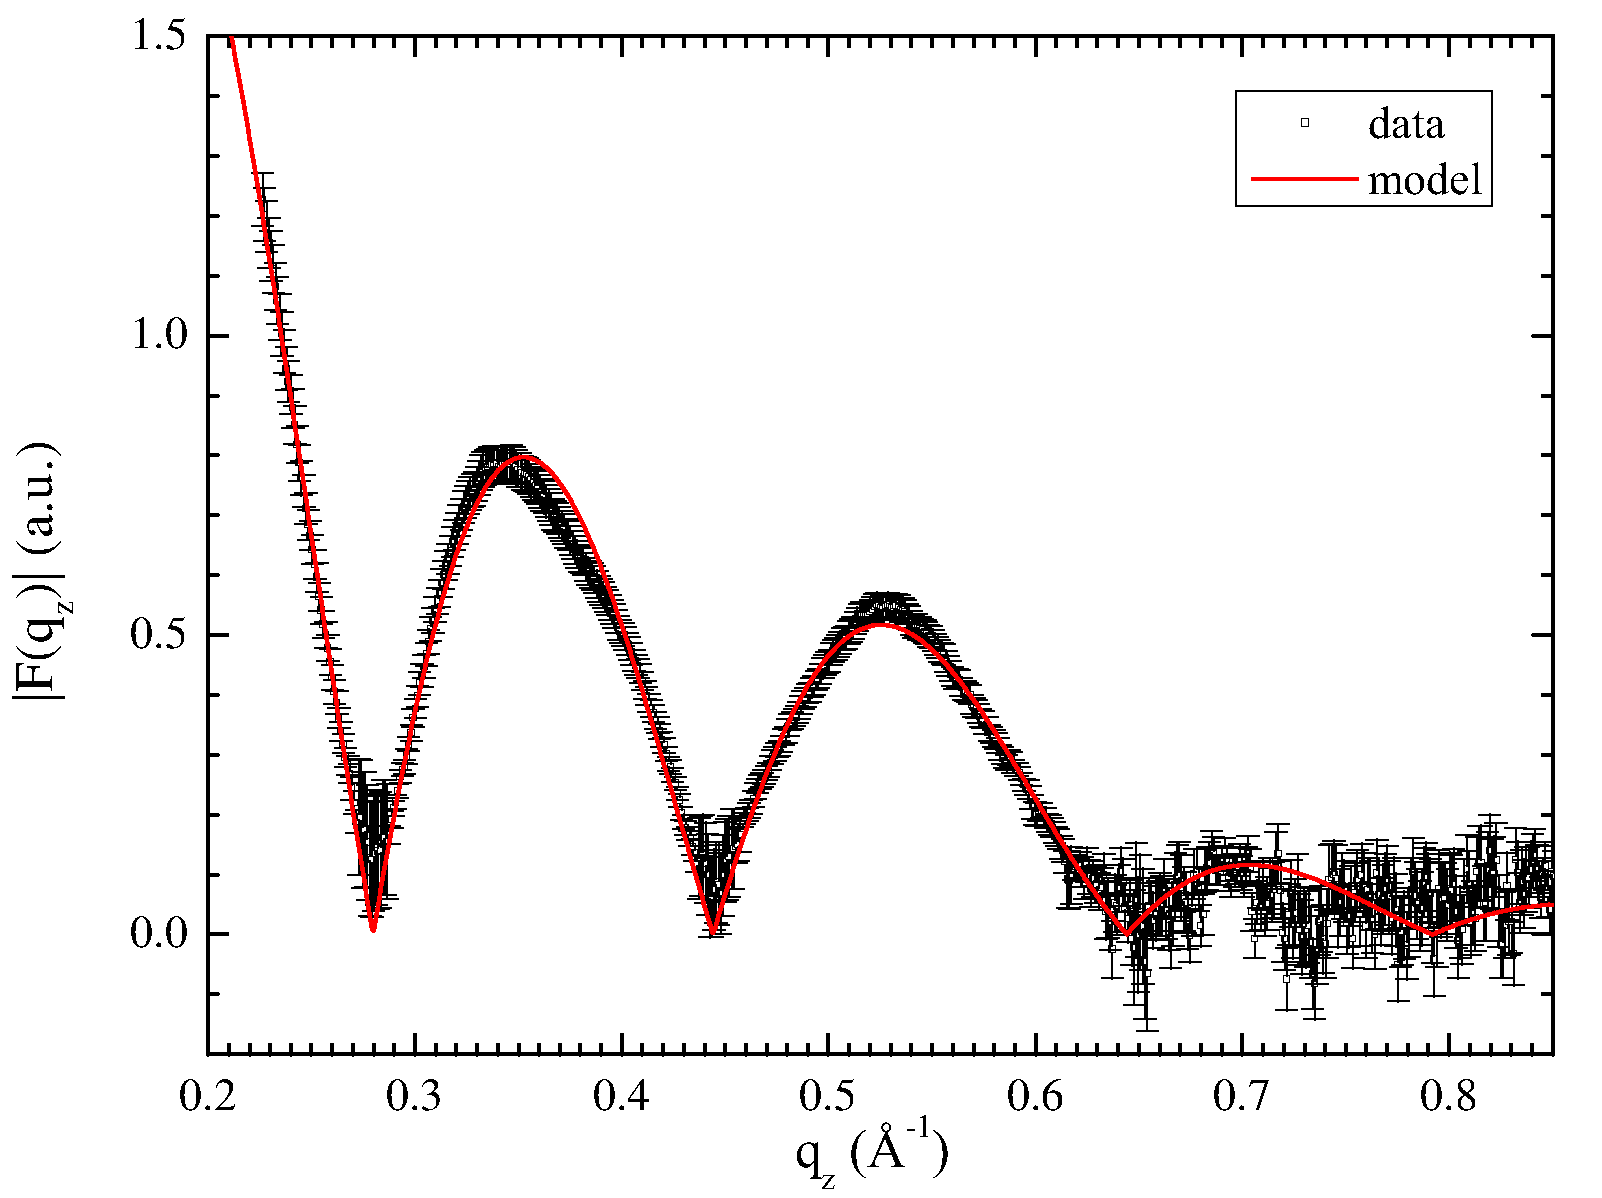
\includegraphics[width=0.45\textwidth,valign=t]{figures/Tat/SDP_Results/XFF/DOPCDOPE3to1_XFF1}
  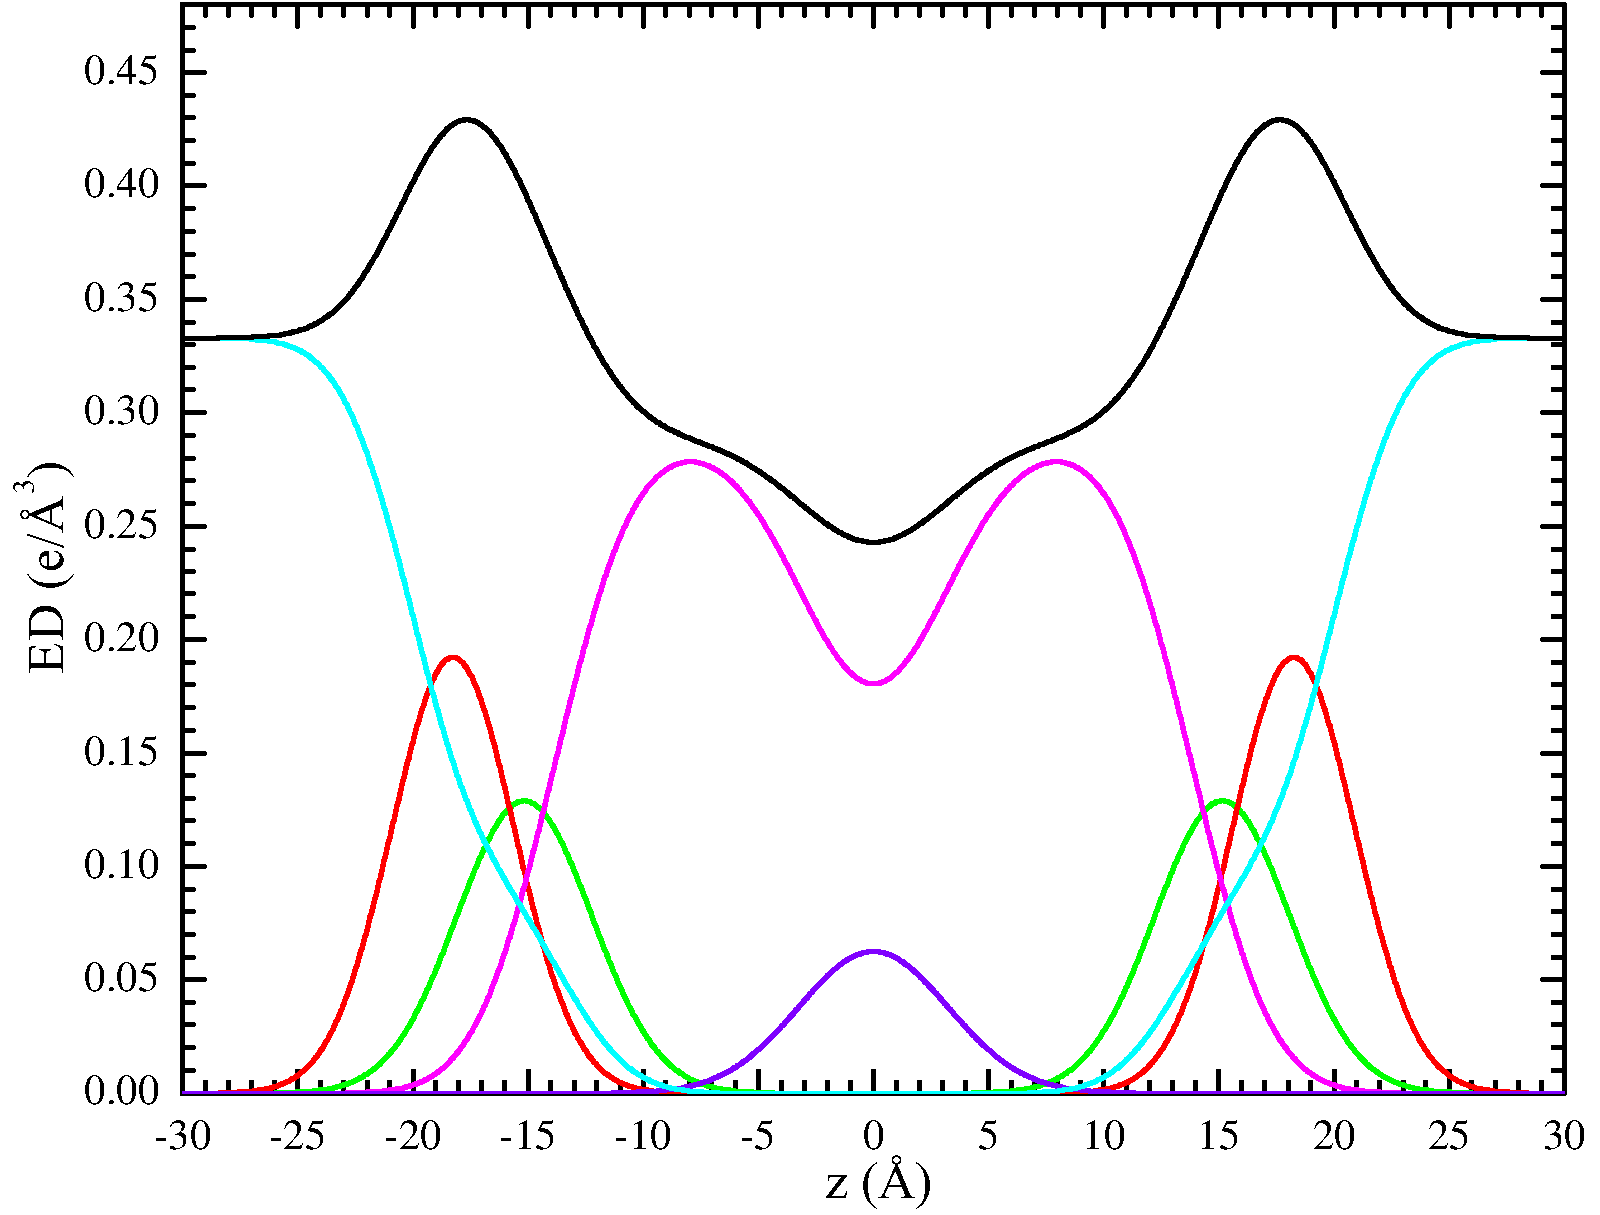
\includegraphics[width=0.45\textwidth,valign=t]{./figures/Tat/SDP_Results/EDP/DOPCDOPE3to1_EDP1}
  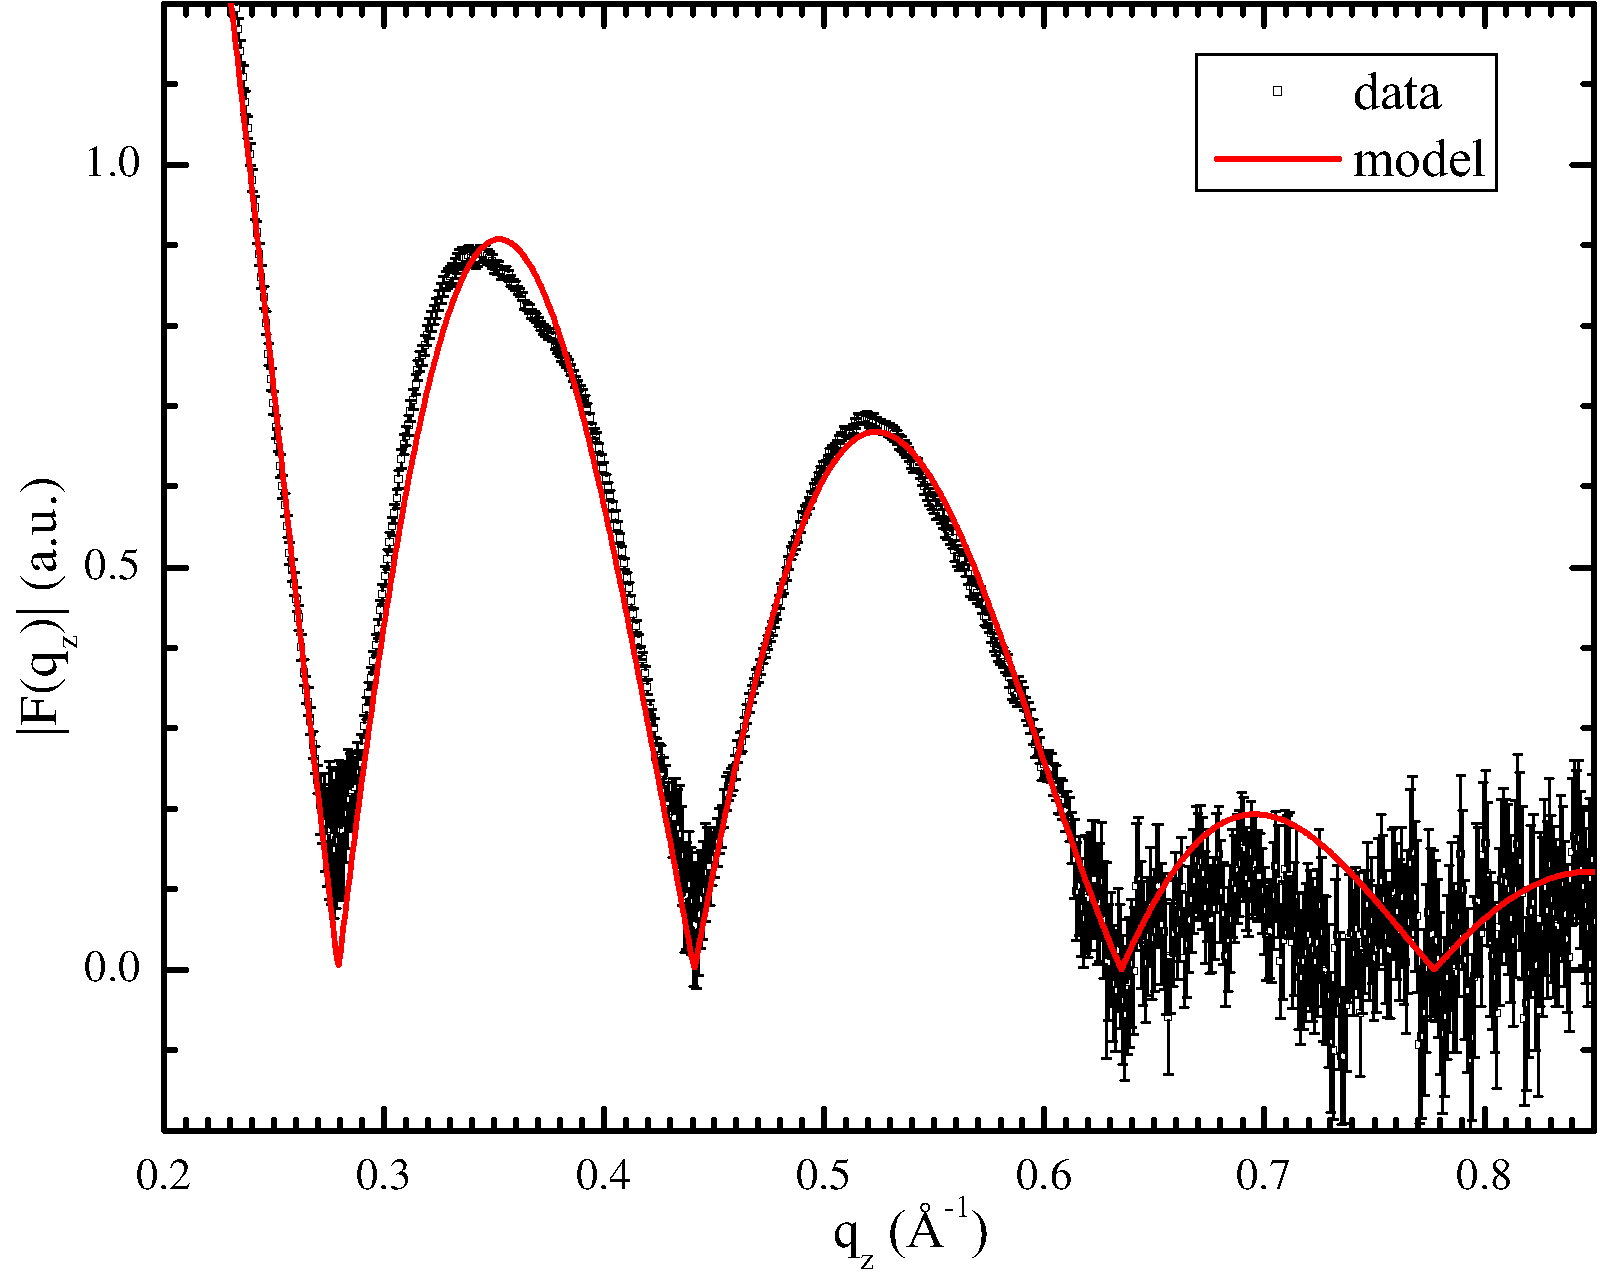
\includegraphics[width=0.45\textwidth,valign=t]{figures/Tat/SDP_Results/XFF/DOPCDOPE3to1_Tat_62to1_3p0_XFF1}
  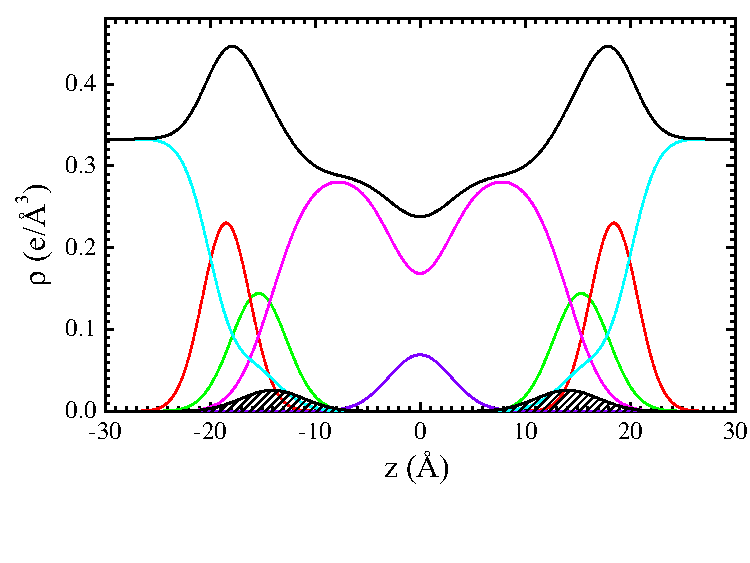
\includegraphics[width=0.45\textwidth,valign=t]{./figures/Tat/SDP_Results/EDP/DOPCDOPE3to1_Tat_62to1_3p0_EDP1}
  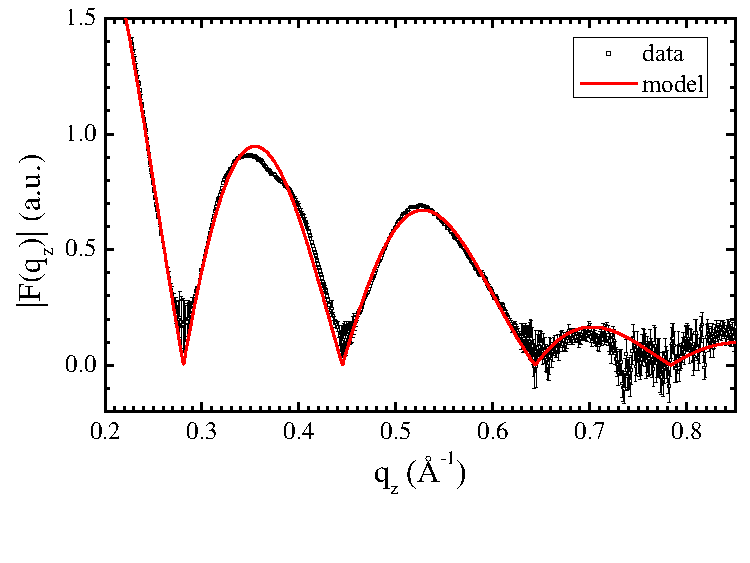
\includegraphics[width=0.45\textwidth,valign=t]{figures/Tat/SDP_Results/XFF/DOPCDOPE3to1_Tat_28to1_3p0_XFF1}
  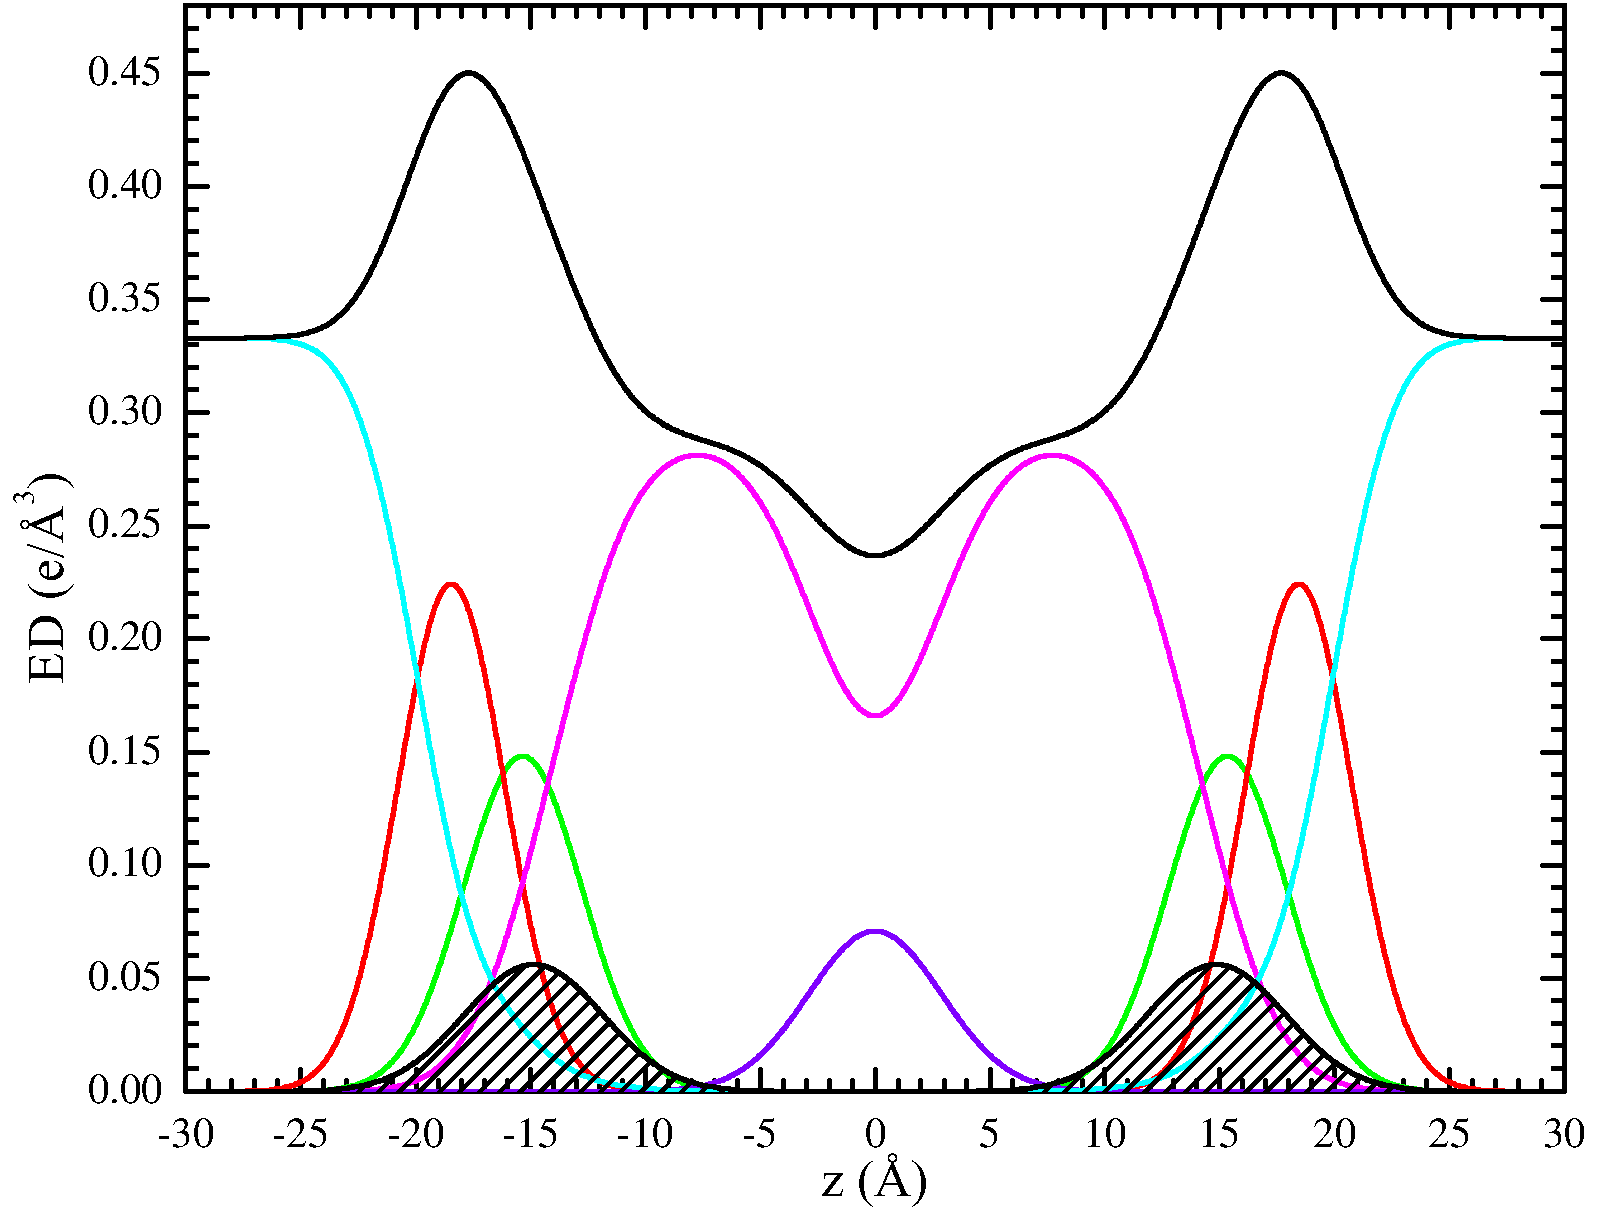
\includegraphics[width=0.45\textwidth,valign=t]{./figures/Tat/SDP_Results/EDP/DOPCDOPE3to1_Tat_28to1_3p0_EDP1}
  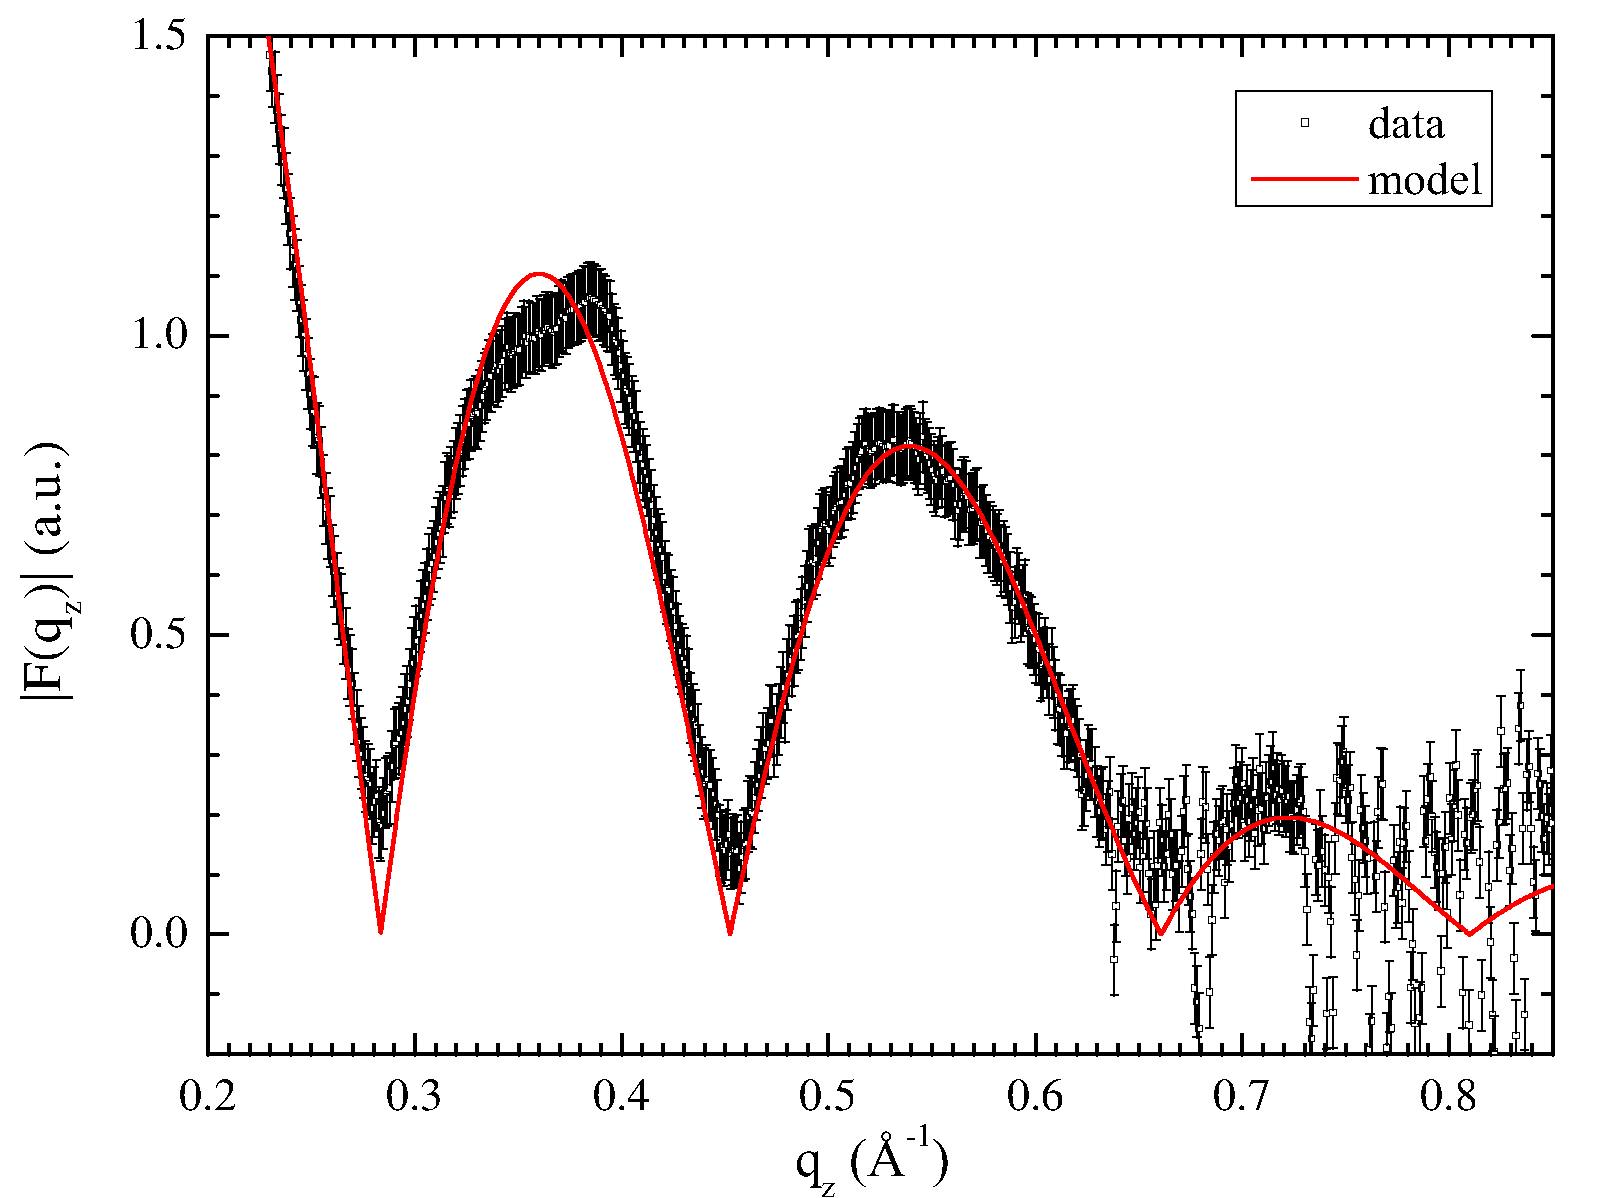
\includegraphics[width=0.45\textwidth,valign=t]{figures/Tat/SDP_Results/XFF/DOPCDOPE3to1_Tat_16to1_3p0_XFF1}
  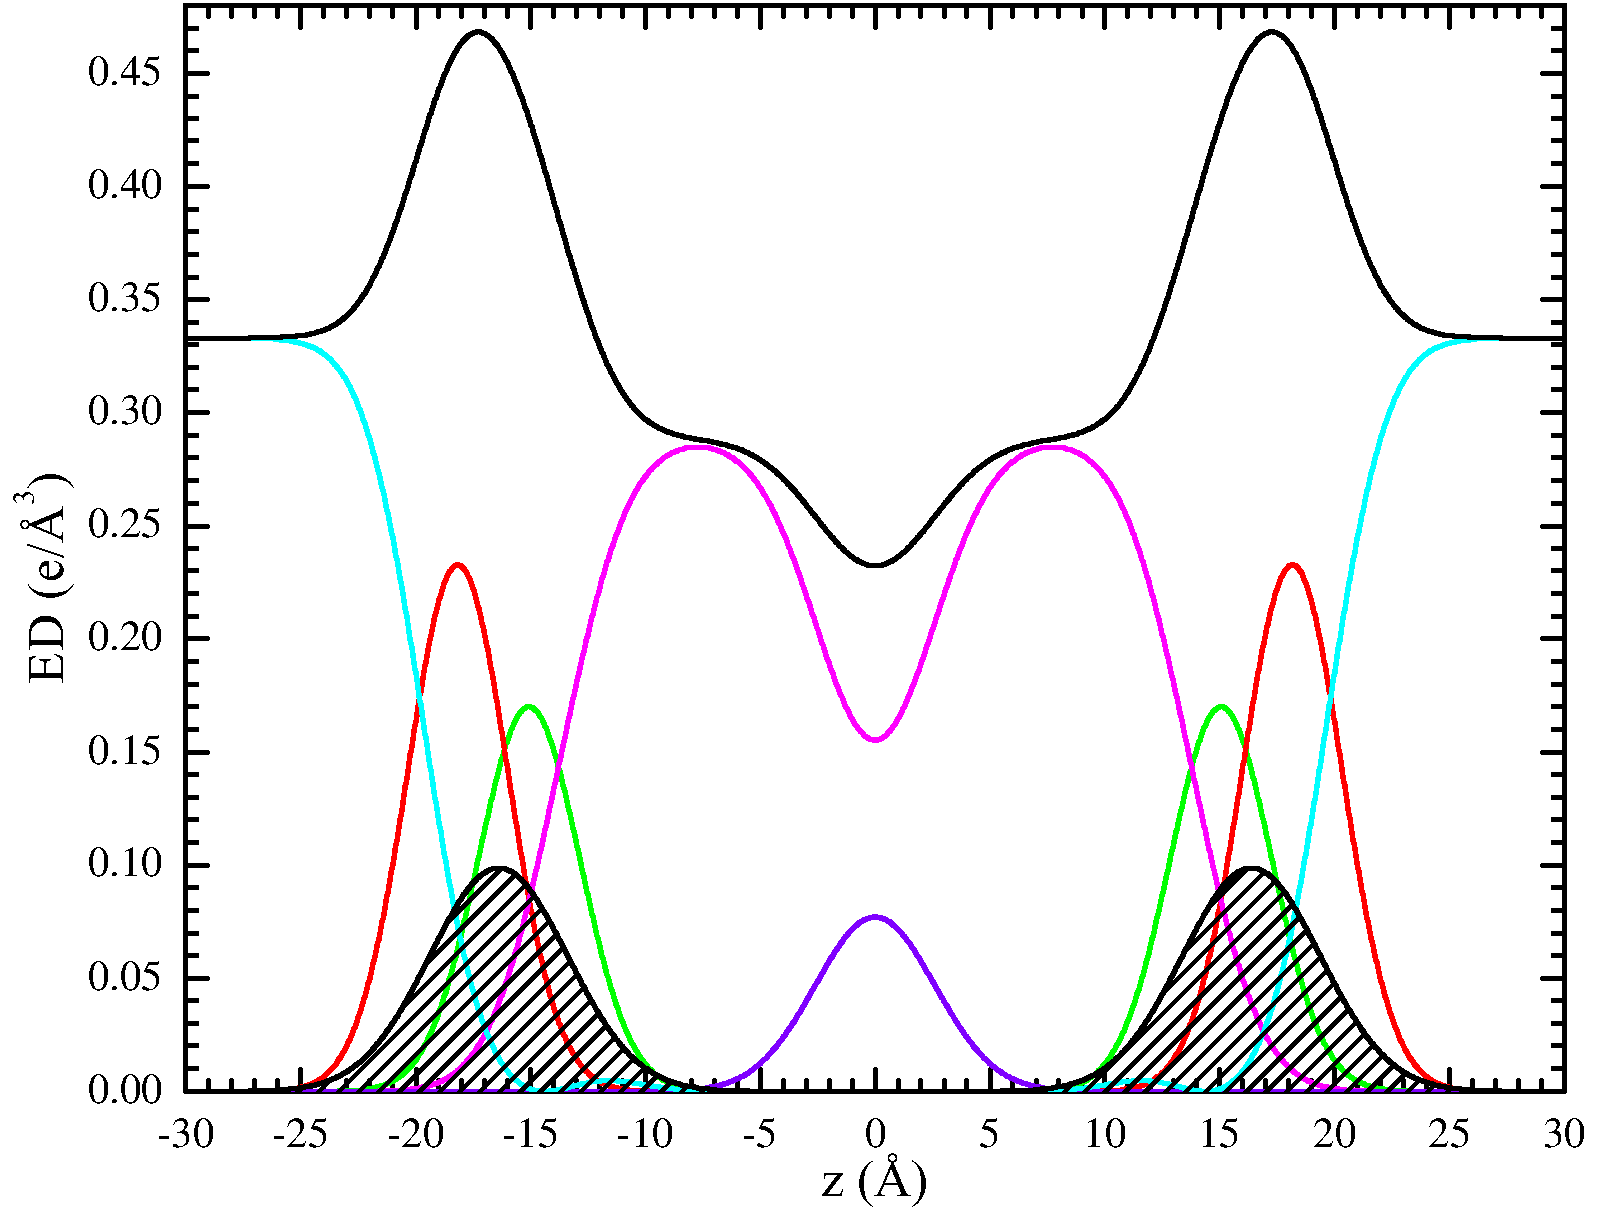
\includegraphics[width=0.45\textwidth,valign=t]{./figures/Tat/SDP_Results/EDP/DOPCDOPE3to1_Tat_16to1_3p0_EDP1}
  \caption{The best fits to DOPC:DOPE (3:1) form factors (left) and the corresponding 
  electron density profiles (right) with $\xTat$ = 0, 0.016, 0.034, 
  and 0.059 (from top to bottom).}
  \label{fig:DOPCDOPE3to1_Tat_XFF1}
\end{figure}

\begin{figure}[htbp]
  \centering
  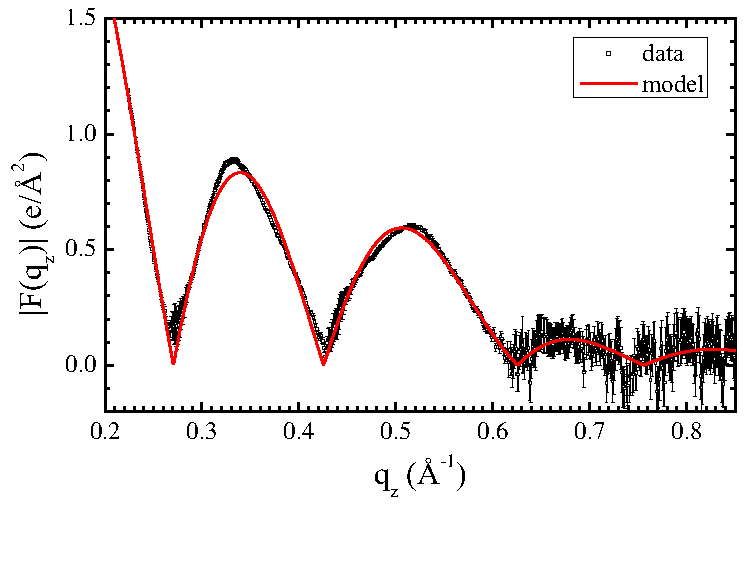
\includegraphics[width=0.45\textwidth,valign=t]{figures/Tat/SDP_Results/XFF/DOPCDOPE1to1_XFF1}
  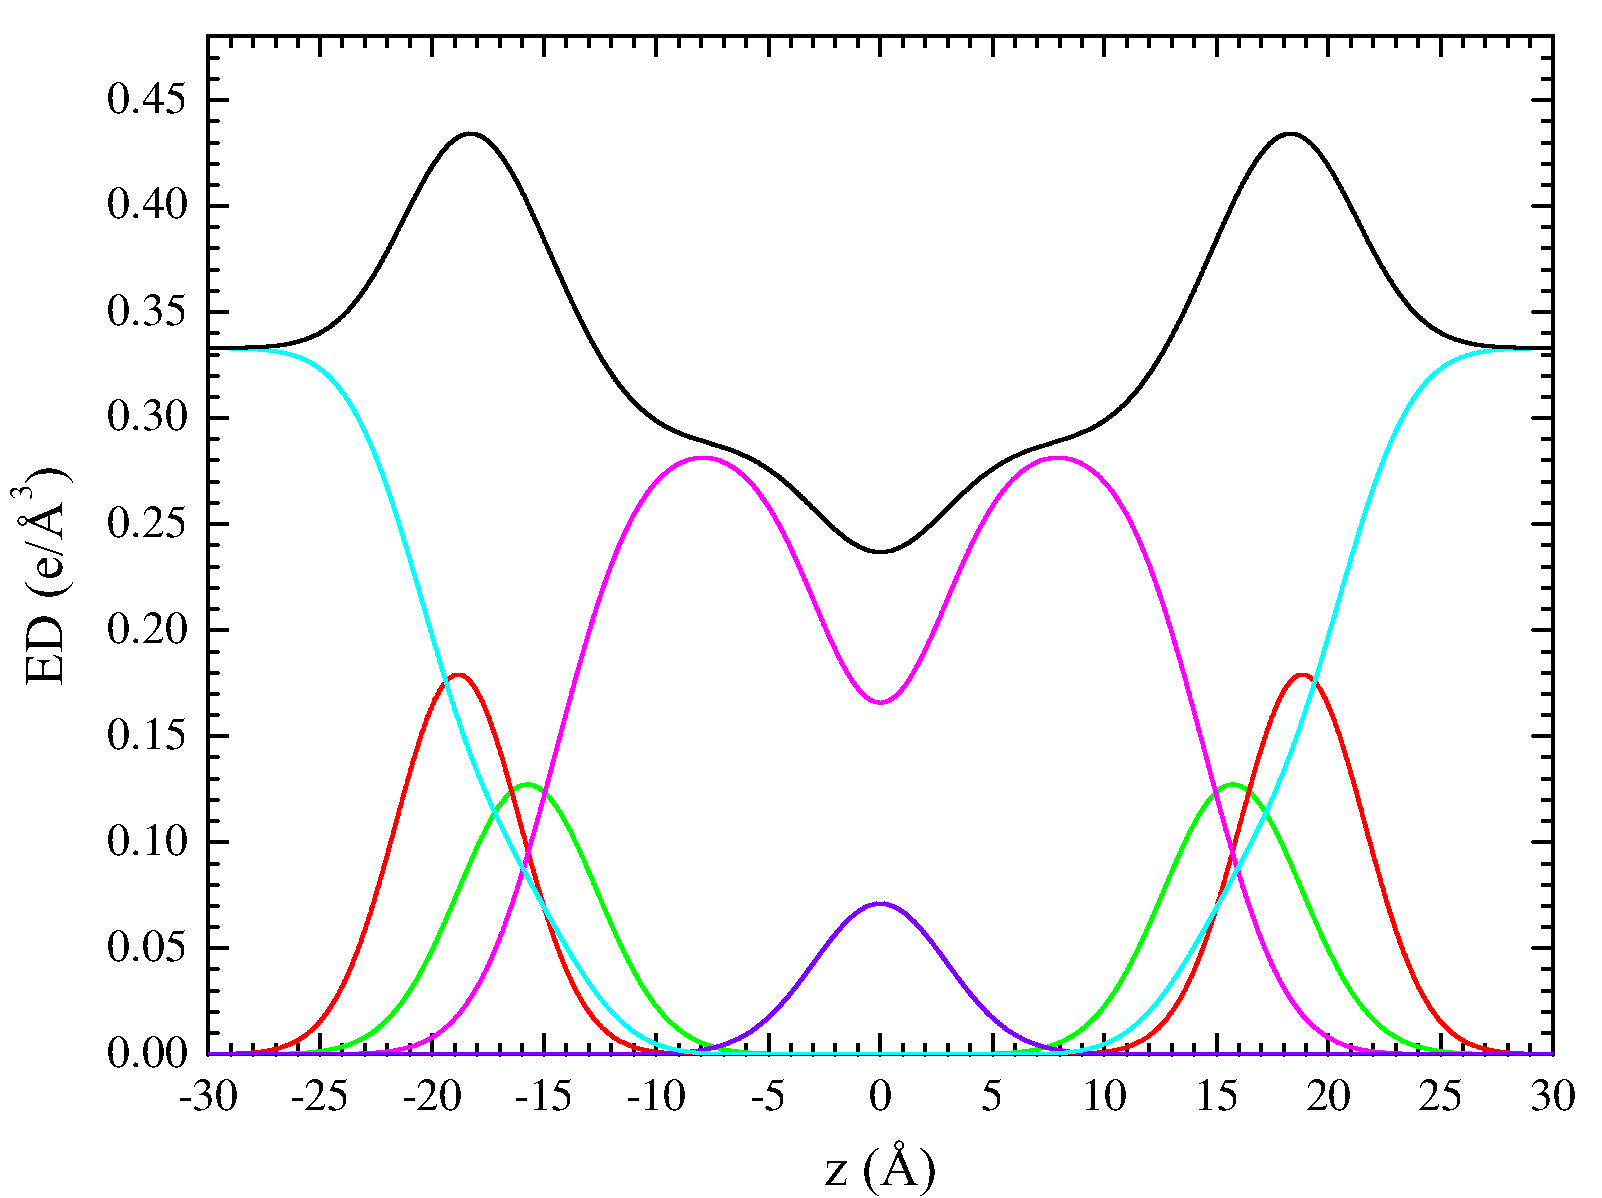
\includegraphics[width=0.45\textwidth,valign=t]{./figures/Tat/SDP_Results/EDP/DOPCDOPE1to1_EDP1}
  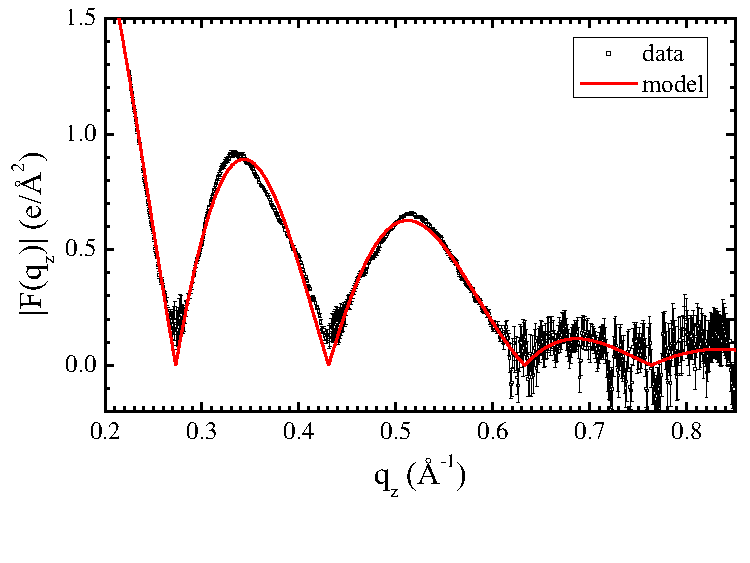
\includegraphics[width=0.45\textwidth,valign=t]{figures/Tat/SDP_Results/XFF/DOPCDOPE1to1_Tat_62to1_3p0_XFF1}
  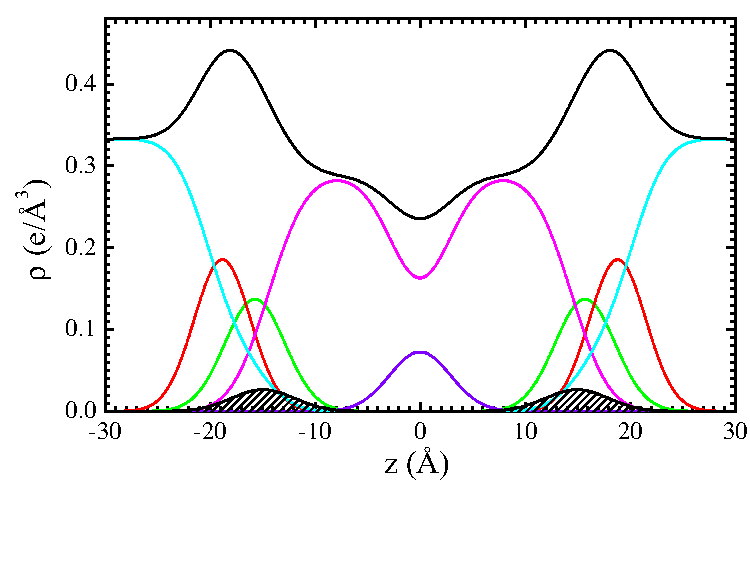
\includegraphics[width=0.45\textwidth,valign=t]{./figures/Tat/SDP_Results/EDP/DOPCDOPE1to1_Tat_62to1_3p0_EDP1}
  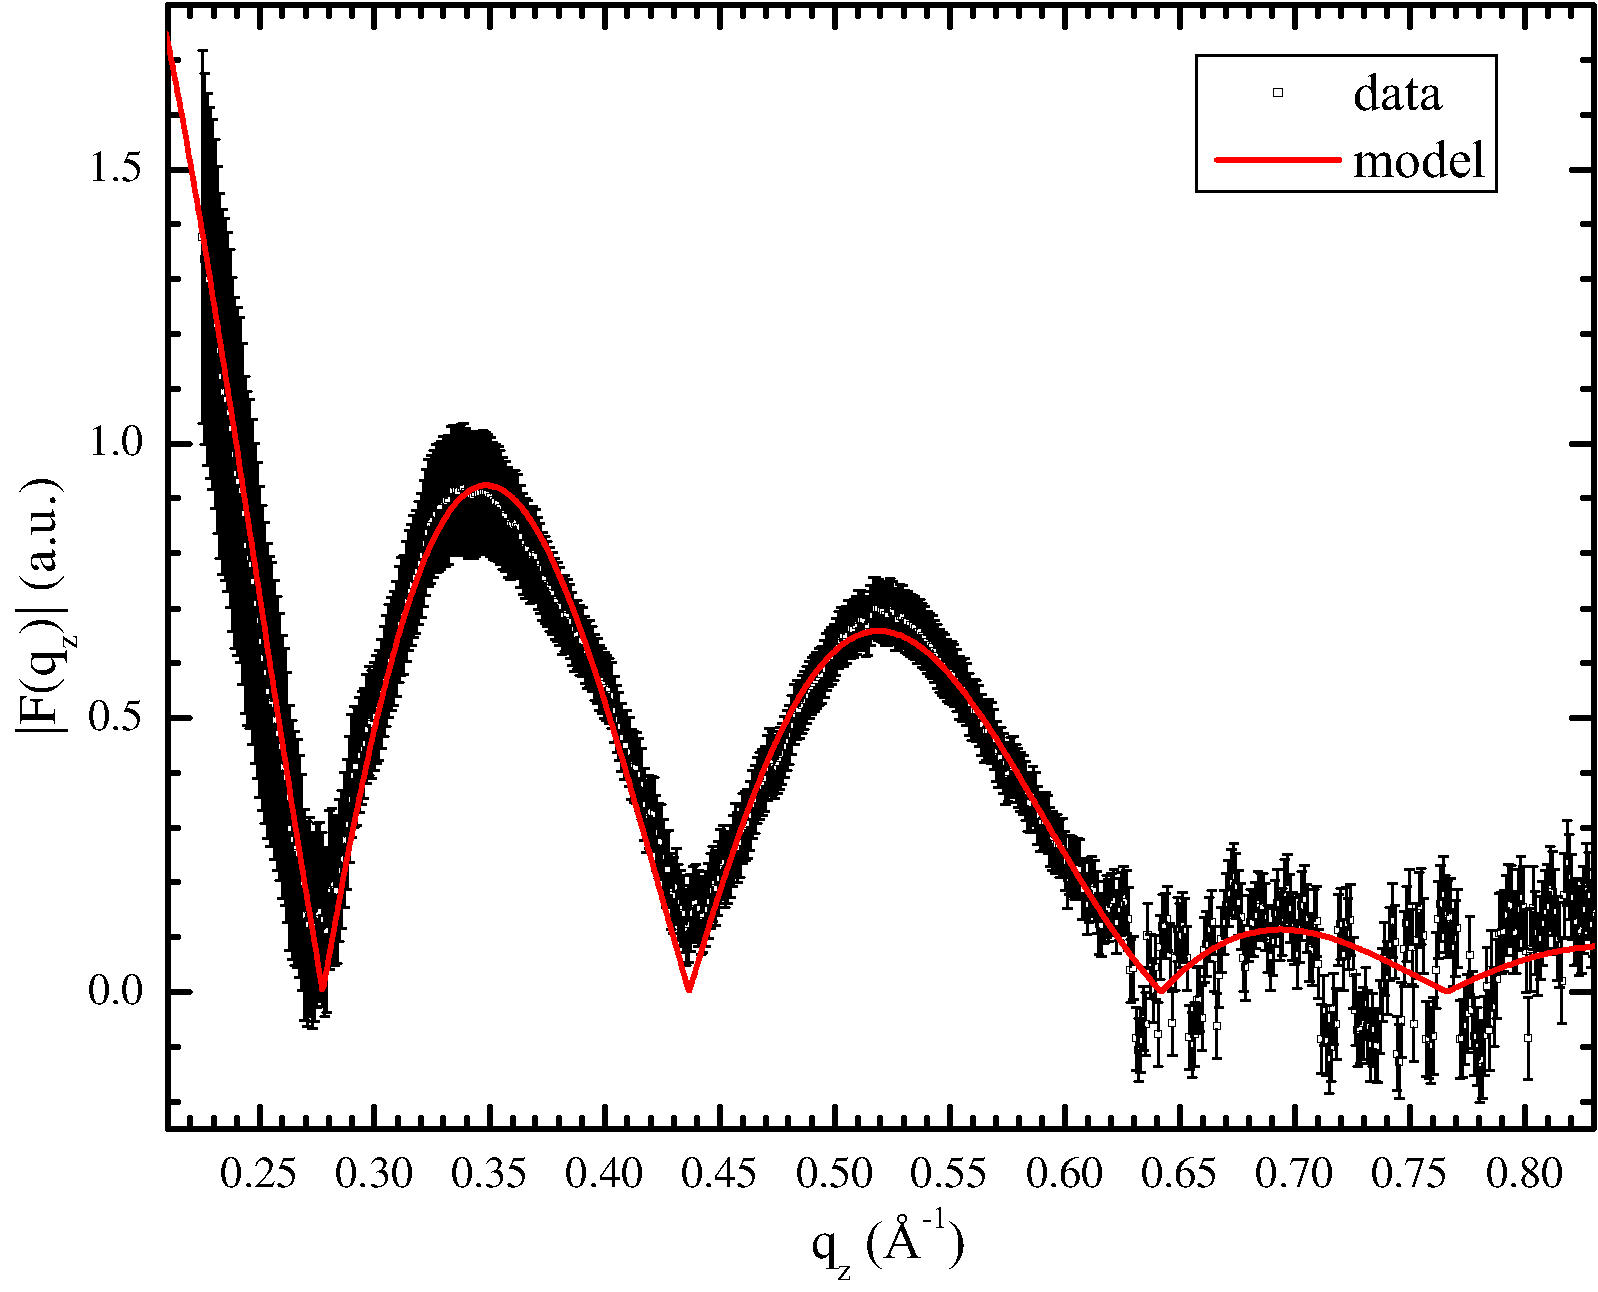
\includegraphics[width=0.45\textwidth,valign=t]{figures/Tat/SDP_Results/XFF/DOPCDOPE1to1_Tat_28to1_3p0_XFF1}
  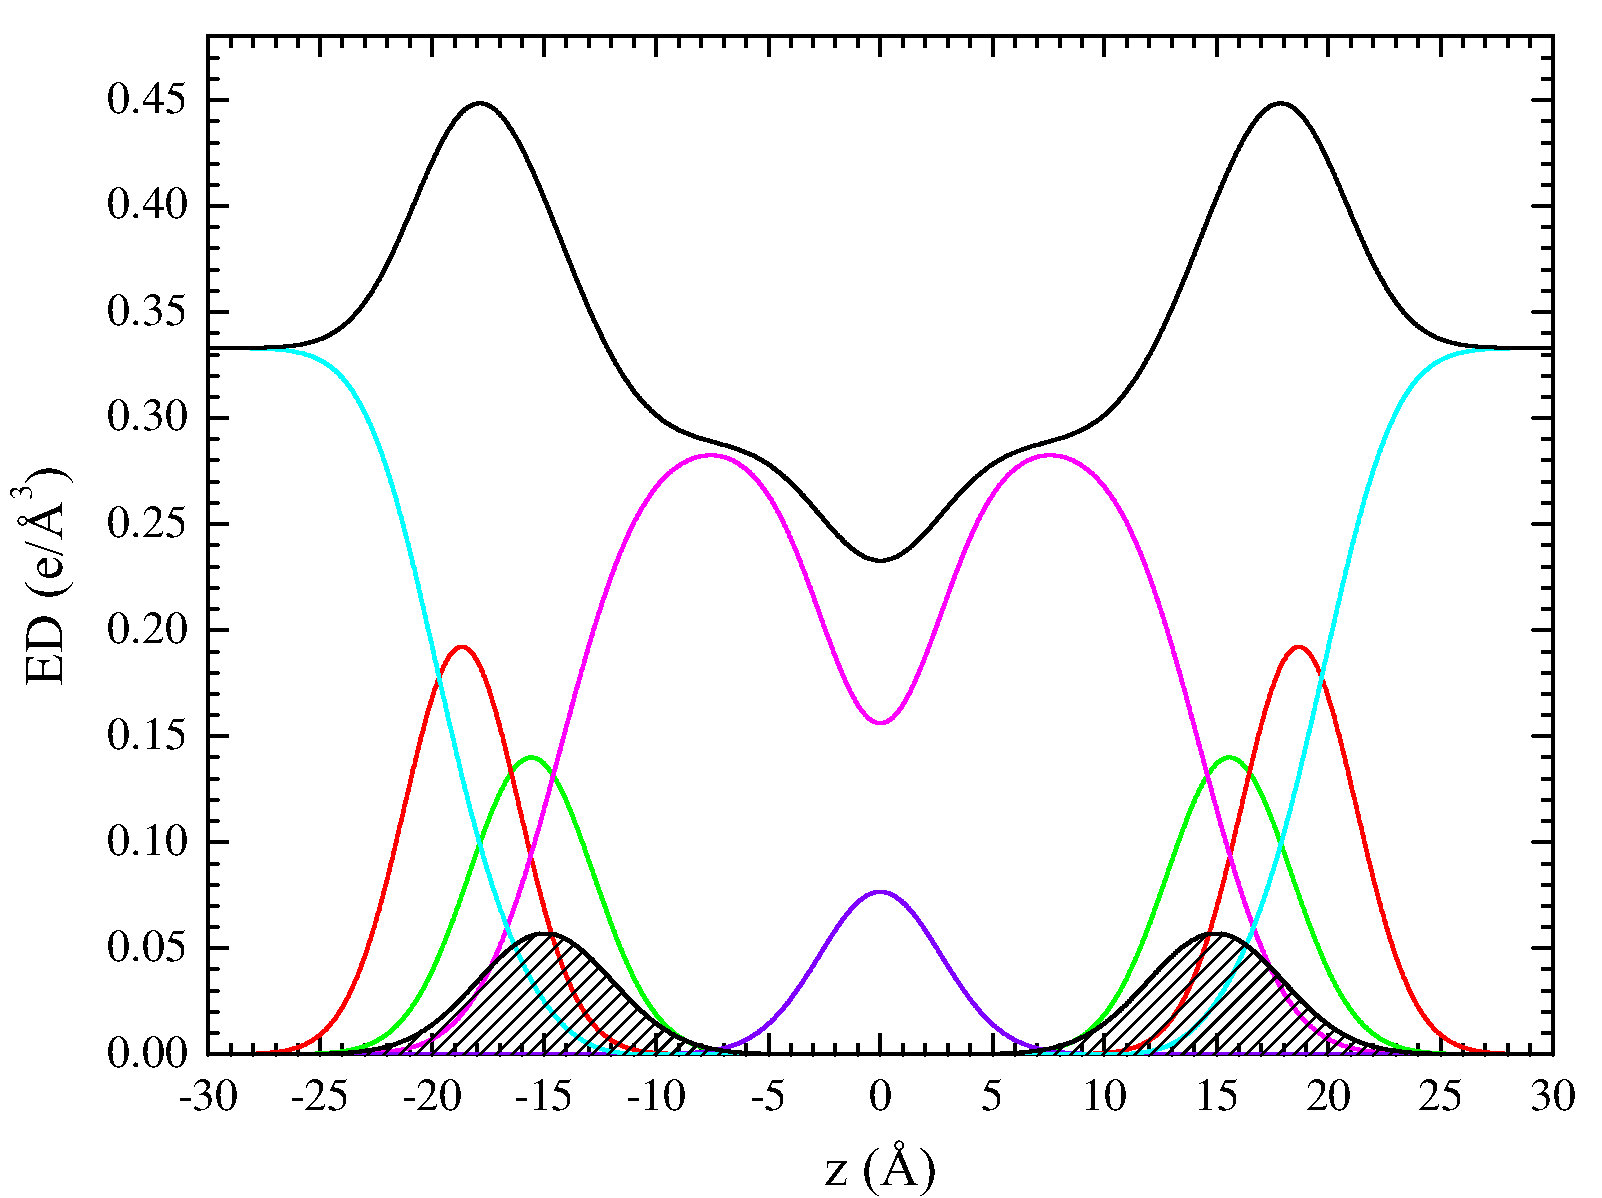
\includegraphics[width=0.45\textwidth,valign=t]{./figures/Tat/SDP_Results/EDP/DOPCDOPE1to1_Tat_28to1_3p0_EDP1}
  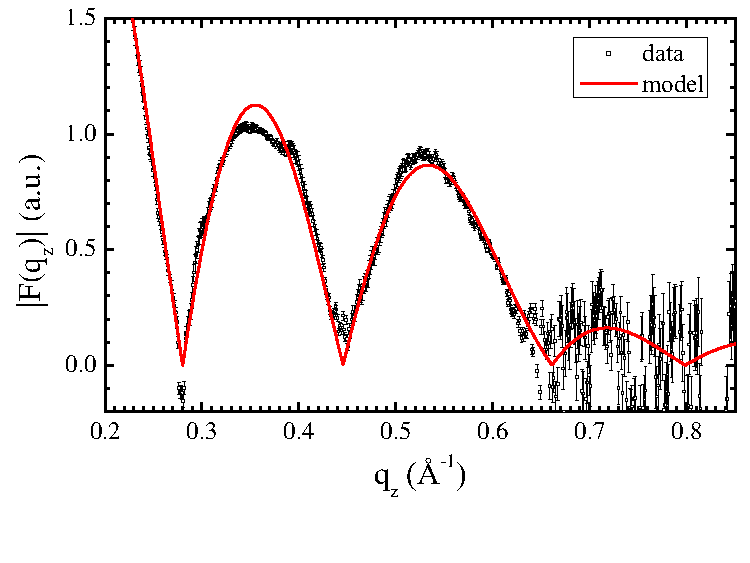
\includegraphics[width=0.45\textwidth,valign=t]{figures/Tat/SDP_Results/XFF/DOPCDOPE1to1_Tat_16to1_3p0_XFF1}
  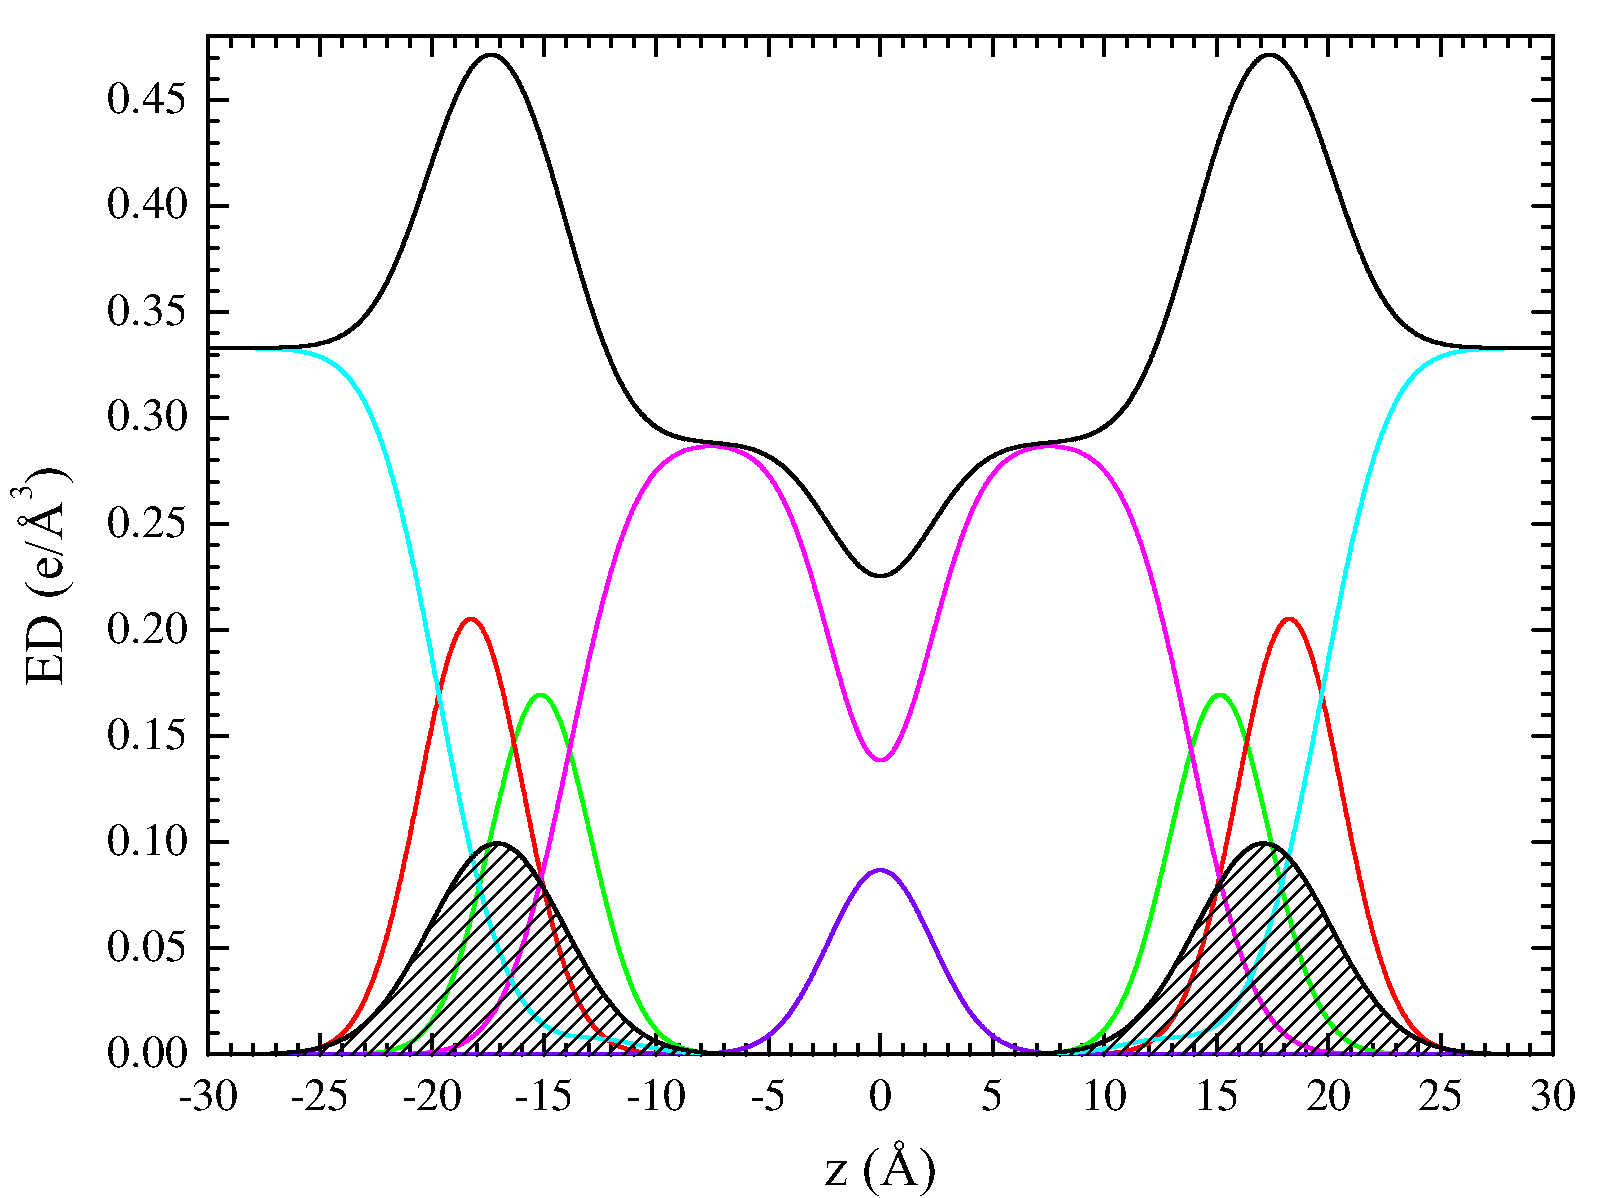
\includegraphics[width=0.45\textwidth,valign=t]{./figures/Tat/SDP_Results/EDP/DOPCDOPE1to1_Tat_16to1_3p0_EDP1}
  \caption{The best fits to DOPC:DOPE (1:1) form factors (left) and the corresponding 
  electron density profiles (right) with $\xTat$ = 0, 0.016, 0.034, 
  and 0.059 (from top to bottom).}
  \label{fig:DOPCDOPE1to1_Tat_XFF1}
\end{figure}

%%%%%%%%%%%%%%%%%%%%%%%%%%%%%%%%%%%%%%%%%%%%%%%%%%%%%%%%%%%%%%%%%%%%%%%%%%%%%%%
\section{Mosaic Spread for NFIT analysis}
\label{sec:mosaic_spread}
First we calculate how mosaic spread affects the structure factor S(q). 
Next we discuss two experimental methods. Third, we discuss the updated NFIT program.
Fourth, we show the results.

\subsection{Mosaic Spread: Calculation}\label{app:mosaic_calc}
In this section, an analytical framework for dealing with mosaic spread is 
developed. A sample of oriented stacks of bilayers consists of many small domains, 
within which layers are registered in an array. 
An ideal domain is a domain where the layers are parallel to the substrate, whose
surface is in the sample $xy$-plane, so
the orientation $\mathbf{n}$ of an ideal domain is perpendicular
to the substrate as shown in Fig.~\ref{fig:spherical_coordinates}.
In general, the orientation $\mathbf{n'}$ of a domain is tilted from that of an
ideal domain by some angle $\alpha$. 
Then, we consider a mosaic spread distribution function, $P(\alpha)$, 
representing a probability of finding a domain with a tilt $\alpha$. 
We assume that the sample is symmetric about the substrate normal, 
so that the distribution $P(\alpha)$ does not depend on the azimuthal angle, $\beta$. 
The normalization condition on $P(\alpha)$ is 
\begin{equation}
  1 = \int_0^{2\pi}\mathop{d\beta}  
      \int_0^{\frac{\pi}{2}}\mathop{d\alpha}\sin\alpha P(\alpha).
\end{equation}
The object of this section is to derive the X-ray scattering structure factor 
including the distribution function $P(\alpha)$. 

\begin{figure}
  \centering
  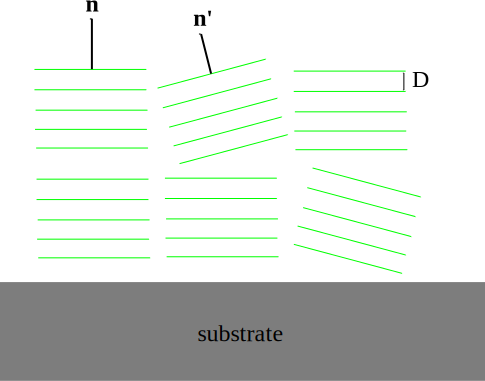
\includegraphics[width=0.65\textwidth]{figures/ripple/mosaic/stack}
  \quad
  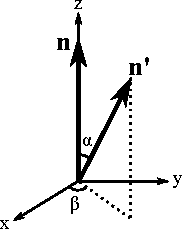
\includegraphics[width=0.25\textwidth]{figures/ripple/mosaic/spherical_coordinates}
  \caption{Two dimensional view of mosaic spread (left) and 
  notations used in this section (right). 
  The stacking direction of an ideal
  domain is $\mathbf{n}$ and that of a tilted domain $\mathbf{n'}$. 
  The deviation of $\mathbf{n'}$ from $\mathbf{n}$ denoted as $\alpha$
  quantifies the degree of misorientation of a domain. 
  The $x$, $y$, and $z$-axes are the sample coordinates.}
  \label{fig:spherical_coordinates}
\end{figure}

First, let us consider a two dimensional example. 
Our sample consists of two identical domains except a tilt $\alpha$
shown in Fig.~\ref{fig:mosaic_2D}.
Then, the sample structure factor $S^\textrm{sam}(\mathbf{q})$ is 
a superposition of the structure factor $S(\mathbf{q})$ of the ideal
domain and $S(\mathbf{q'})$ of the tilted domain,
\begin{equation}
  S^\textrm{sam}(\mathbf{q}) = S(q_x,q_z) + S(q_x',q_z').
  \label{eq:S2D}
\end{equation}
To express $S(q_x',q_z')$ in terms of the sample $q$-space $(q_x,q_z)$, 
we write $q_x'$ and $q_z'$ in terms of $q_x$, $q_z$, and $\alpha$,
\begin{align}
  q_x' &= \mathbf{q}\cdot\xhat' = q\cos\left(\frac{\pi}{2}-\theta+\alpha\right) \nonumber\\
  q_z' &= \mathbf{q}\cdot\zhat' = q\sin\left(\frac{\pi}{2}-\theta+\alpha\right) \nonumber\\
  q_x &= q\cos(\pi/2-\theta) \nonumber\\
  q_z &= q\sin(\pi/2-\theta)
  \label{eq:q2D}
\end{align}
where $q=|\mathbf{q}|$. Eq.~(\ref{eq:S2D}) and (\ref{eq:q2D}) give
the structure factor of a sample consisting of the two domains. With a 
continuous distribution of $\mathbf{n'}$, we integrate over the angle $\alpha$
with each structure factor modulated by the distribution function $P(\alpha)$,
\begin{equation}
  S_M(\mathbf{q})=S_M(q,\theta)=\int_{-\frac{\pi}{2}}^{\frac{\pi}{2}}
  \mathop{d\alpha} S(q_x',q_z')P(\alpha),
  \label{eq:SM2D}
\end{equation}
Variables $q$ and $\theta$ are used in the above equation to make a connection with the
three dimensional case, where the spherical coordinates are convenient, which
we discuss now.

\begin{figure}
  \centering
  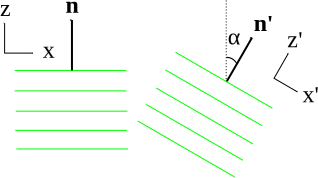
\includegraphics[width=0.55\textwidth]{figures/ripple/mosaic/mosaic_2D}
  \quad\quad
  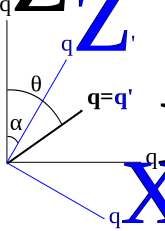
\includegraphics[width=0.25\textwidth]{figures/ripple/mosaic/mosaic_2Dqspace}
  \caption{Example of a two dimensional sample consisting of an ideal
  and tilted domains. $\mathbf{q} = (q_x,q_z)$ is the sample $q$-space and
  $\mathbf{q'} = (q_x',q_z')$ is the domain $q$-space. The two $q$-spaces
  are related by a rotation of $\alpha$ about the $y$-axis, which is into 
  the page.}
  \label{fig:mosaic_2D}
\end{figure}

For a three dimensional sample, the basic idea is the same as the two 
dimensional case. In the three dimensional case, we also rotate the vector $\mathbf{n'}$
about the $z$-axis by an angle $\beta$ after the rotation about the $y$-axis
by an angle $\alpha$, so
all we need to do is to apply appropriate rotation matrices to
the sample $xyz$-axes which define the domain coordinates $x'y'z'$.

The rotation matrix for rotating a vector about the $y$-axis is given by
\begin{equation}
  R_y =  
  \begin{pmatrix} 
    \cos\alpha & 0 & \sin\alpha \\ 
    0 & 1 & 0 \\
    -\sin\alpha & 0 & \cos\alpha 
  \end{pmatrix}
\end{equation}
and for rotating about the $z$-axis
\begin{equation}
  R_z = 
  \begin{pmatrix} 
    \cos\beta & -\sin\beta & 0 \\ 
    \sin\beta & \cos\beta & 0 \\
    0 & 0 & 1 
  \end{pmatrix}.
\end{equation}
Then, what we want is
\begin{equation}
  \mathbf{\hat{x}}' = 
  R_zR_y
  \begin{pmatrix}
    1 \\
    0 \\
    0
  \end{pmatrix}
  = 
  \begin{pmatrix}
    \cos\alpha\cos\beta \\
    \cos\alpha\sin\beta \\
    -\sin\alpha
  \end{pmatrix}
\end{equation}
\begin{equation}
  \mathbf{\hat{y}}' = 
  R_zR_y
  \begin{pmatrix}
    0 \\
    1 \\
    0
  \end{pmatrix}
  =
  \begin{pmatrix}
    -\sin\beta \\
    \cos\beta \\
    0
  \end{pmatrix}
\end{equation}
\begin{equation}
  \mathbf{\hat{z}}' = 
  R_zR_y
  \begin{pmatrix}
    0 \\
    0 \\
    1
  \end{pmatrix}
  =
  \begin{pmatrix}
    \sin\alpha\cos\beta \\
    \sin\alpha\sin\beta \\
    \cos\alpha
  \end{pmatrix}.
\end{equation}
The domain $q$-space, $(q_x',q_y',q_z')$, in terms of the sample $q$-space 
$(q_x,q_y,q_z)$ is given by
\begin{align}
  q_x' &= \mathbf{q} \cdot \mathbf{\hat{x}'} 
  = q_x\cos\alpha\cos\beta + q_y\cos\alpha\sin\beta -q_z\sin\alpha, 
  \label{eq:qx'} \\
  q_y' &= \mathbf{q} \cdot \mathbf{\hat{y}'} 
  = -q_x\sin\beta + q_y\cos\beta, 
  \label{eq:qy'} \\
  q_z' &= \mathbf{q} \cdot \mathbf{\hat{z}'} 
  = q_x\sin\alpha\cos\beta + q_y\sin\alpha\sin\beta + q_z\cos\alpha.
  \label{eq:qz'}
\end{align}
The transformation expressed in the spherical coordinates is 
\begin{align}
  \cos\theta' = \frac{q_z'}{q} 
              = \sin\theta\sin\alpha\cos(\phi-\beta) + \cos\theta\cos\alpha, 
               \label{eq:theta'}\\
  \tan\phi' 
    = \frac{q_y'}{q_x'}
    = \frac{\sin\theta\sin(\phi-\beta)}{\sin\theta\cos\alpha\cos(\phi-\beta) 
                                       -\cos\theta\sin\alpha}.
  \label{eq:phi'}
\end{align}
Summing over all the domains, we get 
for the mosaic spread modified structure factor
\begin{equation}
  S_M(q,\theta,\phi) = \int_0^{2\pi}\mathop{d\beta} \int_0^{\frac{\pi}{2}} 
  \mathop{d\alpha} S(q,\theta',\phi')P(\alpha)
  \label{eq:SM}
\end{equation}
with Eq.\,(\ref{eq:theta'}) and Eq.\,(\ref{eq:phi'}). 

To test these equations, let us apply them to the simple case of 
a stack of rigid layers with their normals parallel to the $z$-axis 
in spherical coordinates.  The structure factor is then
\begin{equation}
  S(q,\theta,\phi) = \frac{\delta(q-\frac{2\pi h}{D})}{q^2} 
  \delta(\cos\theta-1) \delta(\phi)
  \label{eq:Bragg_spherical}
\end{equation}
where $\delta(x)$ is the Dirac delta function. 
From Eq.~(\ref{eq:phi'}), $\delta(\phi')$ is equivalent to
$\delta(\beta-\phi)$. Setting $\beta=\phi$ in Eq.~(\ref{eq:theta'}) gives
$\cos\theta'=\cos(\alpha-\theta)$. 
Then, the mosaic spread modified structure factor $S_M(\mathbf{q})$ is
\begin{align}
  S_M(q,\theta,\phi) &= \int\mathop{d\alpha}\int\mathop{d\beta}
  \frac{\delta(q-\frac{2\pi h}{D})}{q^2} \delta(\cos\theta'-1) \delta(\beta-\phi)P(\alpha) \nonumber\\
  &= \frac{\delta(q-\frac{2\pi h}{D})}{q^2} \int\mathop{d\alpha} \delta(\cos[\alpha-\theta]-1)P(\alpha)\nonumber\\
  &= \frac{\delta(q-\frac{2\pi h}{D})}{q^2}P(\theta).
  \label{eq:SM_Bragg}
\end{align}
Eq.~(\ref{eq:SM_Bragg}) describes hemispherical shells with
radii of $2\pi h/D$ in the sample $q$-space. As will be described
in the next section, a 2D detector records cross sections of these shells,
which give rise to mosaic arcs along $q=2\pi h/D$. 

The structure factor of thermally fluctuating layers is not simple delta functions
and gives rise to diffuse scattering. Analysis of the diffuse scattering 
from a sample with mosaic spread requires Eq.~(\ref{eq:SM}).

\subsection{Mosaic Spread: Near Equivalence of Two Methods}\label{app:mosaic_exp}
In this section, we discuss experimental procedures to probe appropriate 
$q$-space
to measure the mosaic spread distribution, $P(\alpha)$. In our setup, the angle of 
incidence between the beam and substrate, denoted by $\omega$, can be varied. A 
conventional method to measure $P(\alpha)$ is a rocking scan, where
one measures the integrated intensity of a given Bragg peak as a function of 
$\omega$ with a fixed detector position. Another method that takes an advantage
of an area detector \cite{Rodriguez-Navarro07} 
measures the intensity as a function of $\chi$ on a two
dimensional detector (see Fig.~\ref{fig:ring_setup}). This method has been used
to quantify complete pole figures for thin films with fiber texture (isotropic 
in-plane orientation) \cite{Baker10}.
First, we want to compare the two methods mentioned 
above and determine their relationship.

\begin{figure}
  \centering
  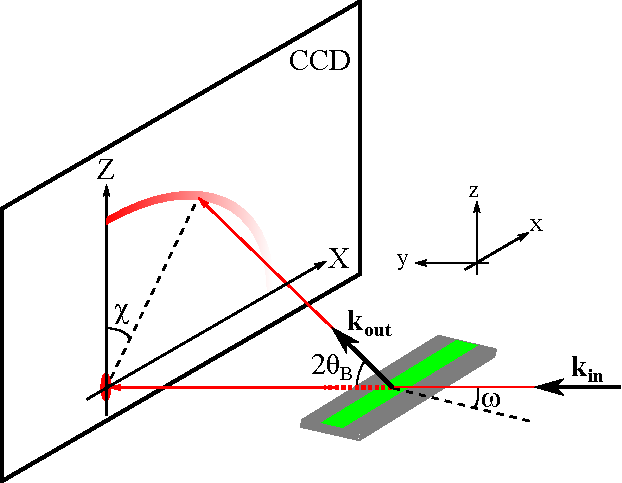
\includegraphics[width=0.8\textwidth]{figures/ripple/mosaic/ring_setup}
  \caption{Notations used in this section. The arc originating from the $Z$-axis
  is the mosaic arc due to the mosaic spread distribution.}
  \label{fig:ring_setup}
\end{figure}

Eq.~(\ref{eq:qxqyqz}) expressed in terms of the coordinates defined in 
Fig.~\ref{fig:ring_setup} is
\begin{align}
  q_x &= q\cos\theta\sin\chi \nonumber\\
  q_y &= q\left(-\sin\theta\cos\omega + \cos\theta\cos\chi\sin\omega\right) \nonumber\\
  q_z &= q\left(\sin\theta\sin\omega + \cos\theta\cos\chi\cos\omega\right).
  \label{eq:ccd2q}
\end{align}
For a rocking scan focused on a particular order, 
$\chi=0$ and $\theta=\theta_B$ while $\omega$ is varied about $\theta_B$, 
where $\theta_B$ is the Bragg angle. Then, 
\begin{align}
  q_x &= 0 \nonumber\\
  q_y &= q_B\sin(\omega-\theta_B) \nonumber\\
  q_z &= q_B\cos(\omega-\theta_B),
  \label{eq:rock} 
\end{align}
which shows that this scan traces a part of the circular path in the $q_x=0$ plane
as shown in Fig.~\ref{fig:rock}. As Fig.~\ref{fig:rock} shows, however, the 
rocking scan only probes a small fraction of the entire distribution, limited
by $2\theta_B$. As discussed in section~\ref{sec:Lorentz_correction}, beyond
$\omega=2\theta_B$, the substrate blocks scattering. On the other hand,
the ring analysis takes advantage of a two dimensional detector and can probe
a substantially wider range of the distribution in principle: approximately $\pm$45\textdegree\
at $\omega=\theta_B$. This method is now described.

\begin{figure}
  \centering
  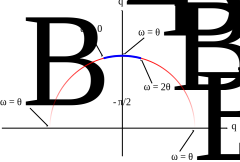
\includegraphics[width=0.7\textwidth]{figures/ripple/mosaic/rock}
  \caption{Rocking scan trace in $q$-space.}
  \label{fig:rock}
\end{figure}

In the ring method, we set $\omega=\theta_B$ and scan on the detector
along $\theta=\theta_B$ as a function of $\chi$. 
Then, Eq.~(\ref{eq:ccd2q}) becomes
\begin{align}
  q_x &= q\cos\theta_B\sin\chi \nonumber\\
  q_y &= q\sin\theta_B\cos\theta_B(\cos\chi-1) \nonumber\\
  q_z &= q(\sin^2\theta_B\ + \cos^2\theta_B\cos\chi),
  \label{eq:ring}
\end{align}
where $q=4\pi\sin\theta_B/\lambda$. For small $\theta_B$, Eq.~(\ref{eq:ring})
reduces to
\begin{align}
  q_x &\approx q\sin\chi \nonumber\\
  q_y &\approx 0 \nonumber\\
  q_z &\approx q\cos\chi.
  \label{eq:ring_small}
\end{align}
For a sharp Bragg peak, this ring method gives the same mosaic intensity 
$I(\chi,\theta_B)$ in Eq.~(\ref{eq:ring_small} as the rocking method mosaic 
intensity $I(\omega - \theta_B)$ in Eq.~(\ref{eq:rock}) because the mosaic 
distribution $P(\alpha)$ is in-plane isotropic. Differences occur when diffuse 
scattering is added.  The diffuse scattering intensity is much broader and weaker 
than the Bragg peaks.  In the ring method, it can be estimated as the average 
from two rings offset on either side from $\theta_B$ and subtracted from the 
$\theta_B$ ring.

\subsection{NFIT}
The original NFIT program was written by Dr. Yufeng Liu and described in his thesis.  
It was used in the Nagle lab, with small updates for data handling, from 2003 until recently.
A newer version has been implemented by Michael Jablin that calculates the theoretical structure factor using 
cylindrical domains appropriate for in-plane correlations \cite{Lyatskaya01}
rather than rectangular domains appropriate for coherence domains. 
All these versions approximated the effect of mosaic spread roughly by averaging 
only in the $q_r$ direction at fixed $q_z$ which means that mosaic rings are approximated 
as mosaic lines or spikes. The subsequent development described here and not yet adopted 
by the Nagle lab calculates the structure factor $S(q_r,q_z)$ with rotational symmetry 
about the $z$-axis, which eliminates the $\phi'$ dependence in Eq.~(\ref{eq:SM}). 
The program interpolates $S(q_r,q_z)$ in terms
of the spherical coordinates $q$ and $\theta$ with $\phi=0$ 
to perform the double integration in Eq.~(\ref{eq:SM}). 
After the mosaic spread integration, the program performs the $q_y$ integration
described in section~\ref{sec:diffuse_analysis}.
For this integration, the calculated $S_M$ is interpolated 
in terms of $q_x$, $q_y$, and $q_z$.

Note: if the structure factor defined in the Cartesian coordinates is desired
(for a case of square domains instead of circular ones),
Eq.~(\ref{eq:qx'} -- \ref{eq:qz'}) can be used instead of 
Eq.~(\ref{eq:theta'}) and (\ref{eq:phi'}).

While it is an improvement, the new program also is an approximation because 
it does not include the unknown form factor $|F(q_z)|$. 
The mosaic spread integration mixes up intensity at different $q_z$ values, so
the separation of $|F(q_z)|$ from $S(\mathbf{q})$ is in principle impossible. 
One way to deal with this issue would be to combine the SDP program, 
which determines $|F(q_z)|$, with the NFIT program, but
that will end up with too many non-linear parameters.
Another possibility is to limit the fitting range to regions close to the meridian.
For a small range of integration, it is not unreasonable to assume that
the form factor is approximately constant as can be seen from 
Eq.~(\ref{eq:qz'}) with small $q_x$, $q_y$, and $\alpha$. 
Therefore, the analysis developed in this appendix ignores the form factor.

%%%%%%%%%%%%%%%%%%%%%%%%%%%%%%%%%%%%%%%%%%%%%%%%%%%%%%%%%%%%%%%%%%%%%%%%%%%%%%%
\newpage
\section{Derivation of the contour part of the form factor}\label{app:FC}
In this section, we derive $\FC$. The ripple profile, $u(x)$ is given by
\begin{equation}
  u(x) = \left\{
    \begin{array}{ccc}
    -\frac{A}{\lambda_r-x_0}\left(x+\frac{\lambda_r}{2}\right) 
      & \text{for} 
      & -\frac{\lambda_r}{2} \leq x < -\frac{x_0}{2} \\
    \frac{A}{x_0}x 
      & \text{for} 
      & -\frac{x_0}{2} \leq x \leq \frac{x_0}{2} \\
    -\frac{A}{\lambda_r-x_0} \left(x-\frac{\lambda_r}{2}\right)
      & \text{for} 
      & \frac{x_0}{2} < x \leq \frac{\lambda_r}{2}
    \end{array} \right.
\end{equation}

The contour part of the form factor is the Fourier transform of the contour
function, $C(x,z)$,
\[
  \FC(\mathbf{q}) = \frac{1}{\lambda_r}
  \int_{-\frac{\lambda_r}{2}}^{\frac{\lambda_r}{2}}\dx
  \int_{-\frac{D}{2}}^\frac{D}{2}\dz 
  C(x,z) e^{iq_zz} e^{iq_xx}
\] 
As discussed in section X, the modulated models allow
the electron density to modulate along the ripple direction, $x$. This means
\begin{align}
  C(x,z) &= \left\{
  \begin{array}{ccc}
    f_1\delta[z-u(x)] & \text{for} & -\frac{\lambda_r}{2} \leq x < -\frac{x_0}{2} \\
    \delta[z-u(x)] & \text{for} & -\frac{x_0}{2} < x < \frac{x_0}{2} \\
    f_1\delta[z-u(x)] & \text{for} & \frac{x_0}{2} \leq x < \frac{\lambda_r}{2} \\    
  \end{array}
  \right. \nonumber\\
  &+ f_2\,\delta\!\pars{x+\frac{x_0}{2}}\delta\!\pars{z+\frac{A}{2}} 
   + f_2\,\delta\!\pars{x-\frac{x_0}{2}}\delta\!\pars{z-\frac{A}{2}}.
\end{align}
The contribution from the minor arm is
\begin{align}
  & \frac{1}{\lambda_r}
  \int_{-\frac{\lambda_r}{2}}^{-\frac{x_0}{2}}\dx e^{iq_xx} e^{iq_zu(x)}
  + \int_{\frac{x_0}{2}}^{\frac{\lambda_r}{2}}\dx e^{iq_xx} e^{iq_zu(x)} \nonumber\\
  &= \frac{1}{\lambda_r}
     \int_{\frac{x_0}{2}}^{\frac{\lambda_r}{2}}\dx 
     e^{-i\left[q_xx-q_z\frac{A}{\lambda_r-x_0}\left(x-\frac{\lambda_r}{2}\right)\right]}
     + \int_{\frac{x_0}{2}}^{\frac{\lambda_r}{2}}\dx 
     e^{i\left[q_xx-q_z\frac{A}{\lambda_r-x_0}\left(x-\frac{\lambda_r}{2}\right)\right]} \nonumber\\
  &= \frac{2}{\lambda_r}
     \int_{\frac{x_0}{2}}^{\frac{\lambda_r}{2}}   
     \cos\bracks{\pars{q_x-q_z\frac{A}{\lambda_r-x_0}}x
                 +q_z\frac{A}{\lambda_r-x_0}\frac{\lambda_r}{2}} \label{eq:minor_arm1}
\end{align}
Using a trigonometric identity, 
\[
  \sin u-\sin v = 2\cos[(u+v)/2]\sin[(u-v)/2],
\]
and defining 
\begin{equation}
  \omega(\mathbf{q}) = \frac{1}{2}\left(q_xx_0 + q_zA\right),
\end{equation}
we further simplify Eq.~(\ref{eq:minor_arm1}),
\begin{align}
  &= \frac{2}{\lambda_r}\frac{\lambda_r-x_0}{\frac{1}{2}q_x\lambda_r - \omega} 
     \cos\bracks{\frac{1}{2}\left(\frac{1}{2}q_x\lambda_r + \omega\right)} 
     \sin\bracks{\frac{1}{2}\left(\frac{1}{2}q_x\lambda_r - \omega\right)} \nonumber\\
  &= \frac{1}{\lambda_r}\frac{\lambda_r-x_0}{\frac{1}{2}q_x\lambda_r - \omega} 
     \cos\bracks{\frac{1}{2}\left(\frac{1}{2}q_x\lambda_r + \omega\right)} 
     \frac{\sin\left(\frac{1}{2}q_x\lambda_r - \omega \right)}
          {\cos\bracks{\frac{1}{2}\left(\frac{1}{2}q_x\lambda_r - \omega\right)}} \nonumber\\
  &= \frac{\lambda_r-x_0}{\lambda_r}
     \frac{\cos\bracks{\frac{1}{2}\left(\frac{1}{2}q_x\lambda_r + \omega\right)}}
          {\cos\bracks{\frac{1}{2}\left(\frac{1}{2}q_x\lambda_r - \omega\right)}}
     \frac{\sin\left(\frac{1}{2}q_x\lambda_r - \omega\right)}
          {\frac{1}{2}q_x\lambda_r - \omega}.
\end{align}
Similarly, we calculate the contribution from the major arm,
\begin{align}
  \frac{1}{\lambda_r}\int_{-\frac{x_0}{2}}^{\frac{x_0}{2}}\dx 
  e^{i\left(\frac{q_zA}{x_0} + q_x \right)x}
  &= \frac{2}{\lambda_r}\int_{0}^{\frac{x_0}{2}}\dx \cos\left(\frac{q_zA}{x_0} + q_x\right)x \nonumber\\ 
  &= \frac{x_0}{\lambda_r}\frac{\sin\omega}{\omega}
\end{align}
The contribution from the kink region is 
\begin{align}
  & \frac{1}{\lambda_r}\iint\dx\dz
  \bracks{\delta\!\pars{x+\frac{x_0}{2}}\delta\!\pars{z+\frac{A}{2}} 
   + \delta\!\pars{x-\frac{x_0}{2}}\delta\!\pars{z-\frac{A}{2}}}
  e^{iq_xx} e^{iq_zz} \nonumber\\
  &= \frac{2}{\lambda_r}\cos\omega.
\end{align}
Therefore,
\begin{align}
  \FC(\mathbf{q}) 
  &= \frac{x_0}{\lambda_r}\frac{\sin\omega}{\omega} + 
  f_1\frac{\lambda_r-x_0}{\lambda_r}
  \frac{\cos\bracks{\frac{1}{2}\left(\frac{1}{2}q_x\lambda_r + \omega\right)}}
       {\cos\bracks{\frac{1}{2}\left(\frac{1}{2}q_x\lambda_r - \omega\right)}}
  \frac{\sin\left(\frac{1}{2}q_x\lambda_r - \omega\right)}
       {\frac{1}{2}q_x\lambda_r - \omega} \nonumber\\
  &+ \frac{2f_2}{\lambda_r}\cos\omega
  \label{eq:FC}
\end{align}

\textcolor{red}{some additional models.} We write the form factor as
\begin{equation}
  F(\mathbf{q}) = F_C^M(\mathbf{q})F_T^M(\mathbf{q}) 
  + f_1F_C^m(\mathbf{q})F_T^m(\mathbf{q}) 
  + f_2F_C^k(\mathbf{q})F_T^k(\mathbf{q})
\end{equation}
such that
\begin{align}
  F_C^M &= \frac{x_0}{\lambda_r}\frac{\sin\omega}{\omega} \\
  F_C^m &= \frac{\lambda_r-x_0}{\lambda_r}
  \frac{\cos\bracks{\frac{1}{2}\left(\frac{1}{2}q_x\lambda_r + \omega\right)}}
       {\cos\bracks{\frac{1}{2}\left(\frac{1}{2}q_x\lambda_r - \omega\right)}}
  \frac{\sin\left(\frac{1}{2}q_x\lambda_r - \omega\right)}
       {\frac{1}{2}q_x\lambda_r - \omega} \\
  F_C^k &= \frac{2}{\lambda_r}\cos\omega.
  \label{eq:FC_split}
\end{align}

%%%%%%%%%%%%%%%%%%%%%%%%%%%%%%%%%%%%%%%%%%%%%%%%%%%%%%%%%%%%%%%%%%%%%%%%%%%%%%%
%\newpage
%\section{Rotation of a Two-Dimensional Function}
%Let us consider rotating a function, $f(x,z)$ in two dimensions by an angle, 
%$\psi$, in the counterclockwise direction (see Fig. X). This is easily 
%achieved by rotating the coordinate system by $\psi$ in the clockwise direction. 
%Let rotated coordinates be $x'$ and $z'$. A point in the original coodinates,
%($x$, $z$), is written as ($x'$, $z'$) in the new coordinates. More specifically,
%the point P is written as 
%$\mathbf{P}=x\xhat+z\zhat=x'\xhat'+z'\zhat'$. $\xhat$ and $\zhat$ in
%the $x'z'$ coordinate system are written as 
%\begin{align}
%  \xhat &= \cos\psi\xhat'+\sin\psi\zhat' \\
%  \zhat &= -\sin\psi\xhat'+\cos\psi\zhat'.
%\end{align}
%Pluggin these in $\mathbf{P}=x\xhat+z\zhat$ leads to
%\begin{align}
%  x' &= x\cos\psi - z\sin\psi \\
%  z' &= z\cos\psi + x\sin\psi,
%\end{align}
%the inverse of which is
%\begin{align}
%  x &= x'\cos\psi + z'\sin\psi \\
%  z &= -x'\sin\psi + z'\cos\psi.
%\end{align}
%Using the latter equations, $f(x,z)$ can be expressed in terms of $x'$ and $z'$. 
%The resulting function $f(x',z')$ is the rotated version of $f(x,z)$. 
%
%As an 
%example, let us consider a Dirac delta function located at $(x,z)=(0,\zh)$,
%that is, $f(x,z)=\delta(x)\delta(z-\zh)$. After the rotation by $\psi$, it 
%becomes
%\begin{align*}
%  f(x,z) 
%  &\rightarrow 
%    \delta(x\cos\psi+z\sin\psi) \delta(-x\sin\psi+z\cos\psi-\zh) \\
%  &= \frac{\delta(x+z\tan\psi)}{|\cos\psi|}
%     \frac{\delta(-x\sin\psi\cos\psi+z\cos^2\psi-\zh\cos\psi)}{1/|\cos\psi|} \\
%  &= \delta(x+z\tan\psi)\delta(z\tan\psi\sin\psi\cos\psi+z\cos^2\psi-\zh\cos\psi) \\
%  &= \delta(x+z\tan\psi)\delta(z-\zh\cos\psi),
%\end{align*}
%which is a part of the expression for $T_\psi(x,z)$ in the simple delta 
%function model.

%%%%%%%%%%%%%%%%%%%%%%%%%%%%%%%%%%%%%%%%%%%%%%%%%%%%%%%%%%%%%%%%%%%%%%%%%%%%%%%
\newpage
\section{Derivation of the transbilayer part of the form factor in the 2G hybrid model}\label{app:FT}
In this section, we derive the trasbilayer part of the form factor calculated
from the 2G hybrid model discussed in Sec.~\ref{sec:LAXS_models}.
Defining $z'=-x\sin\psi+z\cos\psi$, the Fourier transform of a Gaussian function 
along the line tilted from $z$-axis by $\psi$ is
\begin{align}
  & \iint\dz\dx \rhoh{i} \exp\braces{-\frac{(z'-\zh{i})^2}{2\sigmah{i}^2}}
  \delta(x\cos\psi+z\sin\psi)e^{iq_xx}e^{iq_zz} \nonumber\\
  &= \frac{1}{\cos\psi}\int_{-\frac{D}{2}}^{\frac{D}{2}}\dz \rhoh{i} \exp\braces{
    -\frac{(z-\zh{i}\cos\psi)^2}{2\sigmah{i}^2\cos^2\psi} + i(q_z-q_x\tan\psi)z
  } \nonumber \\
  &\approx \rhoh{i}\sqrt{2\pi}\sigmah{i} \,\mathrm{exp}
  \braces{
    i\alpha\zh{i} - \frac{1}{2}\alpha^2\sigmah{i}^2
  } \label{eq:gauss_FT}
\end{align}
with $\alpha=q_z\cos\psi-q_x\sin\psi$.
Using Eq.~(\ref{eq:gauss_FT}) and adding the other side of the bilayer and
the terminal methyl term, we get
\begin{multline}
  F_\mathrm{G} = \sqrt{2\pi}
  \Bigg[
    -\rhom\sigmam \exp\braces{
      -\frac{1}{2}\alpha^2\sigmam^2
    } \\
    + \sum_{i=1}^{1\text{ or }2}2\rhoh{i}\sigmah{i}
    \cos(\alpha\zh{i})
    \,\mathrm{exp}\braces{-\frac{1}{2}\alpha^2\sigmah{i}^2}
  \Bigg].
\end{multline}
The strip part of the 
model in the minus fluid convention is
\begin{equation}
  \rhos(z) = \left\{
    \begin{array}{ccc}
      -\Delta\rho & \text{for } & 0 \leq z < \zchtwo\cos\psi, \\
      0   & \text{for } & \zw\cos\psi \leq z \leq D/2,
    \end{array}
  \right.
\end{equation}
where $\Delta\rho=\rhow-\rhochtwo$.
Then, the corresponding Fourier transform is 
\begin{align}
  F_\mathrm{S} 
  &= \iint\dz\dx e^{iq_xx}e^{iq_zz} \rhos(z)\delta(x\cos\psi+z\sin\psi) \nonumber\\
  &= \frac{2}{\cos\psi} \int_0^{\zchtwo\cos\psi}\dz\cos\pars{\frac{\alpha}{\cos\psi} z}(-\Delta\rho) \nonumber\\
  &= -2\Delta\rho\frac{\sin(\alpha\zchtwo)}{\alpha}.
\end{align} 
The bridging part of the model in the minus fluid convention is 
\begin{align}
  \rhob(x,z) = \frac{\Delta\rho}{2} \cos \bracks{
    \frac{-\pi}{\deltazh}(z'-\zw)} - \frac{\Delta\rho}{2}
\end{align}
for $\zchtwo\cos\psi < z < \zw\cos\psi$, and 0 otherwise. Here,
$\deltazh=\zw-\zchtwo$.
Then, for the strip part of the form factor, we have
\begin{align}
  F_\mathrm{B} 
  &= \iint\dz\dx e^{iq_xx}e^{iq_zz} \delta(x\cos\psi+z\sin\psi) \rhob(x,z) \nonumber\\
  &= \frac{\Delta\rho}{\cos\psi}
     \int_{\zchtwo\cos\psi}^{\zw\cos\psi}\dz \cos\pars{\alpha\frac{z}{\cos\psi}} 
     \braces{\cos\bracks{-\frac{\pi}{\deltazh}\left(\frac{z}{\cos\psi}-\zw\right)} - 1} \nonumber\\
  &= \Delta\rho \braces{
       \frac{\deltazh\sin\bracks{\frac{\pi(-u+\zw)}{\deltazh}+\alpha u}}{-2\pi+2\alpha\deltazh}
       + \frac{\deltazh\sin\bracks{\frac{\pi(u-\zw)}{\deltazh}+\alpha u}}{2\pi+2\alpha\deltazh}
       - \frac{\sin(\alpha u)}{\alpha}  
     }\Bigg|_{\zchtwo}^{\zw} \nonumber\\
  &= -\frac{\Delta\rho}{\alpha}\bracks{\sin(\alpha\zw)-\sin(\alpha\zchtwo)} \nonumber\\
  & \,\quad + \frac{\Delta\rho}{2} \pars{
      \frac{1}{\alpha+\frac{\pi}{\deltazh}} 
      + \frac{1}{\alpha-\frac{\pi}{\deltazh}}
    }\bracks{\sin(\alpha\zw)+\sin(\alpha\zchtwo)}.
\end{align}
Because our X-ray scattering intensity was measured in a relative scale, 
an overall scaling factor was necessary for a non linear least square 
fitting procedure. This means that $\Delta\rho$ can be absorbed in the 
scaling factor. Doing so means that the values of $\rhoh{i}$ and $\rhom$
resulting from a fitting procedure are relative to $\Delta\rho$. One way 
to have these parameters in the absolute scale is to integrate the 
bilayer electron density over the lipid volume and equate the result
to the total number of electrons in the lipid, which can easily be calculated
from the chemical formula. For the ripple phase study in this thesis, the
absolute values of the electron density were not of importance, so the
discussion was omitted in the main text.

%%%%%%%%%%%%%%%%%%%%%%%%%%%%%%%%%%%%%%%%%%%%%%%%%%%%%%%%%%%%%%%%%%%%%%%%%%%%%%%
\newpage
\section{Correction due to refractive index}\label{app:refraction}
$q_z$ needs to be corrected for index of refraction \cite{Liu03}. 

Let $\theta'$ and $\lambda'$ be the true scattering angle and wavelength
within the sample. The wavelength by an energy analyzer, $\lambda$, and the 
scattering angle calculated from a position on a CCD detector, $\theta$ are 
apparent. The correction is not necessary in the horizontal direction.
The Snell's law in Fig. X gives
\begin{align}
  n\cos\theta &= n'\cos\theta' \\
  n\lambda &= n'\lambda'.
\end{align}
For low angle X-ray scattering, the momentum transfer along $z$ direction is
\begin{align}
  q_z &= \frac{4\pi\sin\theta'}{\lambda'} \\
      &= \frac{4\pi n'}{n\lambda}\sin\theta' \\
      &= \frac{4\pi n'}{n\lambda}\sqrt{1-\cos^2\theta'} \\
      &= \frac{4\pi n'}{n\lambda}\sqrt{1-\left(\frac{n}{n'}\cos\theta\right)^2}.
\end{align}
The apparent scattering angle, $\theta$, is directly related to the vertical
pixel position, $p_z$, by 
\begin{equation}
  \theta = \frac{1}{2}\tan^{-1}\left(\frac{p_z}{S}\right),
\end{equation}
where $S$ is the sample-to-detector distance. The typical units of $S$ and 
$p_z$ are in mm. In our experimental setup,
$n=1$ and $n'=0.9999978$ for lipids at $\lambda=1.18$ \AA. 
$S=359.7$ mm.

%%%%%%%%%%%%%%%%%%%%%%%%%%%%%%%%%%%%%%%%%%%%%%%%%%%%%%%%%%%%%%%%%%%%%%%%%%%%%%%
\newpage
\section{Thin Rod Model of the ripple phase}
The thin rod model will be applied to the ripple phase WAXS. 
In this model, electron density of lipid chains are described as delta 
functions and lipid head groups are assumed not to contribute to scattering. 
Since the molecular packing of the major side of ripple phase is hypothesized 
to be gel-like, the model may be adequate. First, we will study diffraction 
from chains packed in gel phase manner whose system size is infinite but whose 
packing plane make an angle $\xi$ with the $xy$ plane. 
This infinite case is adequate for indexing the ripple Bragg peaks while
it ignores the peak broadening effect.
The system will later be truncated along the ripple direction to see the effect 
of the finite size on peak broadening. Finally, in-plane powder will be taken 
into account to derive a peak intensity pattern.

First, let us calculate the positions of the diffraction peaks from a two 
dimensional orthorhombic lattice whose plane makes an angle $\xi$ with 
respect to the $xy$ plane and extends to infinity. 
As a unit cell, we will take a parallelpipedon containing two rods,
one located at the origin and the other located at the center
(Fig.~\ref{fig:unit_cell_waxs}).
The lattice vectors are $\mathbf{a_1}=a_1\cos\xi\xhat+a_1\sin\xi\zhat$ 
and $\mathbf{a_2}=a_2\yhat$. \textcolor{red}{There are other choices for
how the lattice is oriented with respect to the ripple direction,
which should be considered as well.}
Then, the Laue conditions are given by
\begin{align}
	2\pi h &=\mathbf{q}\cdot\mathbf{a_1}=(a_1\cos\xi)q_x+(a_1\sin\xi)q_z \\
	2\pi k &=\mathbf{q}\cdot\mathbf{a_2}=a_2 q_y,
\end{align}
with $h$ and $k$ being zero or integer. 
Let us define the chain tilt angle $\theta$ to be the angle between
the stacking $z$ direction and the chain direction. We also define
$\phi$ to represent the direction into which chains are tilted.
In other words, $\theta$ and $\phi$ are usual spherical coordinates
with respect to the ripple $x$, $y$, and $z$ axes, not the local
bilayer Cartesian axes. With this choice of coordinates, chains 
are tilted with respect to the local bilayer normal if 
$\theta$ = 0. $\theta=\xi$ and $\phi=\pi$ gives chains parallel to the
local bilayer normal, or $\theta_t$ = 0. 
\textcolor{red}{It would be good to work out
the relation between $\theta$ and $\theta_t$, $\theta_t$ being the chain tilt
with respect to the local bilayer normal.}

\begin{figure}
  \centering
  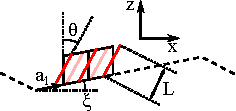
\includegraphics[width=0.6\textwidth]{figures/ripple/unit_cell_waxs_side} \\
  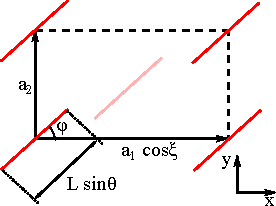
\includegraphics[width=0.6\textwidth]{figures/ripple/unit_cell_waxs_top}
  \caption[Unit cell for chain packing in the major arm]
  {Unit cell for chain packing in the major arm. 
  (top) Projection of the unit cell in the $xz$-plane. The unit cell is taken
  as a parallelpipedon shown by black solid lines, each unit cell 
  containing two chains.
  Chains located at the center of the unit cell are
  drawn as opaque red lines while chains at the lattice points are 
  drawn as solid red lines. The dash line indicates
  the mid-plane of a rippling bilayer. Chains are tilted with respect to
  the stacking $z$ direction by $\theta$ and the major arm is tilted 
  with respect to the ripple $x$ direction by $\xi$. The chain length
  is denoted by $L$. $\mathbf{a_1}$ and $\mathbf{a_2}$ are orthorhombic 
  unit cell vectors.
  (bottom) Projection of the unit cell in the $xy$-plane.
  $\phi=0$ means chains are tilted in the $xz$ plane and $\phi=\pi/2$
  means chains are titled into the direction perpendicular to the 
  ripple direction.}
  \label{fig:unit_cell_waxs}
\end{figure}

The electron density, assuming a delta function for each chain, is given by 
\begin{align}
	\rho(\mathbf{r})&=\delta(x-\alpha z, y-\beta z)+\\
	&\delta\left[x-\frac{a_1\cos\xi}{2}-\alpha\left(z-\frac{a_1\sin\xi}{2}\right),\, y-\frac{a_2}{2}-\beta\left(z-\frac{a_1\sin\xi}{2}\right)\right],
\end{align}
where $\alpha=\tan\theta\cos\phi$ and $\beta=\tan\theta\sin\phi$. The first rod extends for
\begin{align}%Range of extension of first rod
	-L/2\sin\theta\cos\phi\leq &x\leq L/2\sin\theta\cos\phi\\ 
	-L/2\sin\theta\sin\phi\leq &y \leq L/2\sin\theta\sin\phi\\
	-L/2\cos\theta\leq &z \leq L/2\cos\theta,
\end{align}
and the second rod for
\begin{align}%Range of extension of second rod
	-L/2\sin\theta\cos\phi+a_1/2\cos\xi\leq &x\leq L/2\sin\theta\cos\phi+a_1/2\cos\xi\\ 
	-L/2\sin\theta\sin\phi+a_2/2 \leq &y \leq L/2\sin\theta\sin\phi+a_2/2\\
	-L/2\cos\theta+a_1/2\sin\xi \leq &z \leq L/2\cos\theta+a_1/2\sin\xi.
\end{align}
Then, the form factor is given by
\begin{align}%form factor calculation
	F(\mathbf{q})&=\int dx\int dy\int dz\,\rho(\mathbf{r})\,e^{i\mathbf{q}\cdot\mathbf{r}}\\
	&=\int_{-\frac{L}{2}\cos\theta}^{\frac{L}{2}\sin\theta}dz e^{i(\alpha q_x+\beta q_y+q_z)z}\,+\nonumber\\
	&\int_{-\frac{L}{2}\cos\theta+\frac{a_1}{2}\sin\xi}^{\frac{L}{2}\cos\theta+\frac{a_1}{2}\sin\xi}dz\, e^{\frac{i}{2}\left[q_x\left(a_1\cos\xi-\alpha a_1\sin\xi\right)+q_y\left(a_2-\beta a_1\sin\xi\right)\right]}\,e^{i(\alpha q_x+\beta q_y+q_z)z}\nonumber\\
	&=\left[1+e^{\frac{i}{2}\left(a_1\cos\xi q_x+a_1\sin\xi q_z+a_2q_y\right)}\right]\frac{2}{\gamma}\sin\left(\frac{\gamma L\cos\theta}{2}\right)\nonumber\\
	&=\left[1+e^{i\pi(h+k)}\right]\frac{2}{\gamma}\sin\left(\frac{\gamma L\cos\theta}{2}\right)\label{eq:FormFactor},
\end{align}
where $\gamma=\alpha q_x+\beta q_y+q_z$. Eq. \ref{eq:FormFactor} shows that peaks with $h+k$ being odd is extinct. For $h+k$ even, we have
\begin{equation}%form factor for even h+k
	F(\mathrm{q})=\frac{4}{\gamma}\sin\left(\frac{\gamma L\cos\theta}{2}\right)\label{eq:FormFactorEven}.
\end{equation} 

For (20) peak, $q_y$ = 0 and $4\pi=a_1\cos\xi q_x+a_1\sin\xi q_z$. The second equation can be rewritten to give
\begin{equation}
	q_z=-\frac{1}{\tan\xi}q_x+\frac{4\pi}{a_1\sin\xi}
\end{equation}
which defines a straight line in $q_xq_z$-plane along which (20) Bragg rod appears. Eq. \ref{eq:FormFactorEven} has a peak at $\gamma$ = 0. Hence, the maximum intensity of (20) peak is at $q_x$ and $q_z$ that satisfy Laue conditions and $\gamma$ = 0. This gives three equations and three unknowns. Explicitly written, we have
\begin{align}
	q_y &= 0\\
	4\pi &= a_1\cos\xi q_x+a_1\sin\xi q_z\\
	0 &= \tan\theta\cos\phi q_x+q_z
\end{align}
Solving these, we get
\begin{align}%q_x and q_z equations for (20) peak
	q_x &= \frac{4\pi}{a_1\cos\xi(1-\tan\theta_t\cos\phi\tan\xi)}\\
	q_z &= \frac{-4\pi\tan\theta_t\cos\phi}{a_1\cos\xi(1-\tan\theta_t\cos\phi\tan\xi)}
\end{align}
For $\phi$ = $\pi$/2, we have $q_x=4\pi/(a_1\cos\xi)$ and $q_z=0$, so one would expect to see a peak on the equator, the case of which is similar to $L_{\beta I}$ phase in gel phase. To get back to ordinary gel phase, $\xi$ should be set equal to zero.

For any (hk) line, we again have three equations and three unknowns as
\begin{align}
	2\pi h &= q_xa_1\cos\xi +q_za_1\sin\xi\\
	2\pi k &= q_ya_2\\
	0 &= q_x\tan\theta_t\cos\phi + \frac{2\pi k}{a_2}\tan\theta_t\sin\phi +q_z
\end{align}
Solving for $q_x$, $q_y$, and $q_z$, we obtain
\begin{align}
	q_x &= \frac{2\pi(h+ka\beta\sin\xi)}{a_1\cos\xi(1-\alpha\tan\xi)}\\
	q_y &= \frac{2\pi k}{a_2}\\
	q_z &= \frac{-2\pi(h\alpha+ka\beta\cos\xi)}{a_1\cos\xi(1-\alpha\tan\xi)},
\end{align}
where $a=a_1/a_2$.